\chapter{Lösungsdetails}
    \label{chapter:SolutionDetails}
    Bisher erfolgte lediglich eine oberflächliche Beschreibung des \glspl{wccs},
    um einen übersichtlichen Blick auf die Konzepte und das System als Ganzes
    zu vermitteln.
    Dieses Kapitel beschreibt das \gls{wccs} nun detaillierter,
    um die Lösung und ihre Umsetzung vollständig zu präsentieren.

    % Spezifikation zur Beschreibung von REST Schnittstellen: https://www.openapis.org/

    \section{Eine domänenspezifische Sprache zur Spezifikation von Klassen}
    Das \gls{wccs} braucht für die Durchführung einer Klassifizierung
    eine Spezifikation, die die bekannten Klassen definiert.

    Hierzu bietet das \gls{wccs} eine domänenspezifsche Sprache:
    Die \gls{wccdl}.

    \subsection{Funktionen}
        Die Sprache greift die in Kapitel \ref{section:conceptClassesFeaturesSelectors}
        beschriebenen Konzepte auf.

        Zunächst erlaubt sie die Definition von benannten Klassen,
        wobei sie die Unterscheidung zwischen Seiten-, Inhalts und Referenzklassen
        erlaubt.
        Des Weiteren kann mit ihr ein Selektor für eine Klasse definiert werden,
        was im Falle von Seitenklassen zwingend erforderlich ist.

        Zu einer Klasse gehören wie beschrieben auch Features,
        die mit der \gls{wccdl} ebenfalls deklariert werden können.
        Neben dem Namen und der Klasse des Features, gehört dazu auch
        ein Selektor und ob es sich um ein mehrelementiges Feature handelt oder nicht.

        % TODO: Muss hier nochmal erwähnt werden, dass der Selektor optional ist?
        % TODO: Muss hier schon darauf hingewiesen werden, dass die Ermittlung ob Content oder ReferenceFeature anhand der Klasse passiert?

    \subsection{Generierungsergebnis}
        Anstatt in ein ausführbares Programme, wird Spezifikation in eine Konfigurationsdatei für
        das Klassifizierungssystem übersetzt.
        Die Sprache ist deklarativ, weshalb keine Anweisungen formuliert werden.
        Der übergeordnete Algorithmus ist deshalb immer gleich.
        Die Programme wärend deshalb zu großen Teilen identisch und unnötig komplex.
        Deshalb sinnvoller ihn auszulagern und Spezifikation lediglich in ein anderes Format zu übersetzen.
        % TODO: Kann das hier vielleicht lieber in die Einleitung. Dann ggf. ohne Begründung?

    \subsection{Vorteile}
        Die Verwendung einer DSL hat mehrere Vorteile.

        \paragraph{Erleichterte Konfiguration des Systems}
        Das technische Format der Konfigurationsdatei wird verborgen
        und die Spezifikation in einem lesbaren Format gespeichert.
        Das erlaubt die Formulierung der Klassendefinitionen prinzipiell auch
        Nicht-Programmierern.
        Selektoren müssen beispielsweise nicht für das technische Format manuell escaped werden,
        was ihre Formulierung erleichtert.

        \paragraph{Fehlervermeidung}
        Dadurch, dass wir mit einer Sprache arbeiten, die in ein Artefakt generiert wird,
        können Fehler besser abgefangen werden.
        Z. B. durch syntaktische Korrektheit oder semantische Validitätsprüfungen.
        Ein Beispiel sind die zur Verfügung stehenden Selektoren und ihre semantisch korrekte Verwendung.
        Genauso kann sichergestellt werden, dass für jedes Feature ein Selektor ableitbar ist.

        \paragraph{Leichtere Wiederverwendbarkeit}
        Durch die logische und physische Aufteilung können Klassendefinitionen leichter
        wiederverwendet oder übertragen werden, als dies bei der direkten Verwendung eines
        technischen Formates wäre.

        \paragraph{Unabhängigkeit vom konkreten Klassifizierungssystem}
        Die Sprache ist unabhängig von der konkreten Implementierung des Klassifizierungssystem.
        Es ist deshalb möglich für verschiedene Implementierungen verschiedene Dateien zu generieren.
    \section{Der Classification Service}
    \label{section:solutionDetailsClassificationService}
    Der Classification Service ist die Komponente im \gls{wccs},
    die die tatsächliche Klassifizierung durchführt.
    Dieses Kapitel widmet sich ein paar Details dieses Services
    und beschreibt seine Arbeitsweise.

    \subsection{Funktionen und Schnittstellen}
    \label{section:solutionDetailsAnnotationServiceFunctions}
    Der {\annotationService} implementiert vor allem die
    Annotator Storage API \cite[Kapitel "`Storage"']{annotator:documentation},
    um die Nutzung dieser Bibliothek zu ermöglichen.
    Gleichzeitig ist seine Schnittstelle allgemein gehalten,
    sodass sie auch von anderen Systemen sinnvoll genutzt werden kann.
    Die Beschreibung der einzelnen Funktionen erfolgt in diesem Kapitel.

    \paragraph{Format einer Annotation}
    Annotationen tauscht der Service über JSON-Dokumente aus,
    die dem Format von Annotator \cite[Kapitel "`Annotation format"' ]{annotator:documentation} folgen.
    Der Service ergänzt aber einige Angaben.
    Das Schema einer Annotation zeigt Listing \ref{listing:annotationServiceAnnotationFormat}.

    \lstinputlisting[
        label=listing:annotationServiceAnnotationFormat,
        caption=Das Format einer Annotation,
        style=json
    ]{../resources/annotation-service/annotation.json}

    Jede Annotation spiegelt genau ein Feature der Klassifikation wider.
    Die ID einer Annotation wird vom {\annotationService} automatisch
    generiert.
    Das Feld \texttt{text} bestimmt den Inhalt der Annotation,
    der hier immer der Namen des Features und dessen Klasse ist.
    Die Angaben im Feld \texttt{ranges} spiegeln den eindeutigen Selektor des Features wider.
    Durch das Feld \texttt{user} identifiziert Annotator den Ersteller der Annotation,
    der in diesem Fall immer der imaginäre technische Benutzer \texttt{wccs} ist.
    Im Feld \texttt{permissions} werden die Rechte \texttt{admin} und \texttt{delete} auf diesen Nutzer beschränkt.
    Jeder Anwender kann dadurch Annotation lesen und bearbeiten.
    Änderungen an den Rechten sowie das Löschen einer Annotation bleibt aber dem Nutzer \texttt{wccs} vorbehalten.
    Die Eigenschaft \texttt{wccs} ist nicht durch Annotator vorgegeben,
    sondern stellt eine Ergänzung des \glspl{wccs} dar.
    Es speichert die Klasse und Art (Inhalt oder Referenz) eines Features.

    \paragraph{Bereitstellung von Informationen über die Schnittstelle}
    Um der Annotator Storage API \cite[Kapitel "`Storage"' ]{annotator:documentation} zu genügen,
    muss ein Endpunkt existieren,
    der Informationen über die Version der implementierten Schnittstelle
    enthält.
    Die entsprechende Schnittstelle ist in Tabelle
    \ref{table:annotationServiceMetaInterface} dokumentiert.

    \begin{table}[htb]
        \centering
        \begin{tabular}{|l|l|}
            \hline
            \textbf{\gls{url}} & \texttt{http://<HOST>:16612/pages/<PAGE\_ID>}\\
            \hline
            \textbf{Methode} & \texttt{GET}\\
            \hline
            \textbf{Statuscode} & \texttt{200 (OK)}\\
            \hline
            \textbf{Ausgabedokument} & \lstinputlisting[title=AnnotationServiceMetaInfo]{../resources/annotation-service/meta.json}\\
            \hline
        \end{tabular}
        \caption{Die Schnittstelle zum Abfragen von Informationen über den {\annotationService}}
        \label{table:annotationServiceMetaInterface}
    \end{table}

    Annotator erwartet von der konfigurierten Datenhaltung,
    dass sie die Annotationen genau einer Seite enthält.
    Die Anfrage-\gls{url} enthält deshalb die \gls{url} der klassifizierten Webseite,
    deren Annotationen angefordert werden.

    \paragraph{Annotationen einer Seite abrufen}
    Zentrale Aufgabe des {\annotationService}s ist die Bereitstellung der Annotationen einer Seite.
    Hierfür bietet der Service die in Tabelle \ref{table:getAllAnnotationsInterface}
    dargestellte Schnittstelle.

    \begin{table}[htb]
        \centering
        \begin{tabular}{|l|l|}
            \hline
            \textbf{\gls{url}} & \texttt{http://<HOST>:16612/pages/<PAGE\_ID>/annotations}\\
            \hline
            \textbf{Methode} & \texttt{GET}\\
            \hline
            \textbf{Statuscode} & \texttt{200 (OK)}\\
            \hline
            \textbf{Ausgabedokument} & \texttt{Array von Annotationen}\\
            \hline
        \end{tabular}
        \caption{Die Schnittstelle zum Abfragen aller Annotationen einer Klassifikation}
        \label{table:getAllAnnotationsInterface}
    \end{table}

    Die Anfrage-\gls{url} identifiziert die klassifizierte Seite,
    an deren Annotationen Interesse besteht,
    über ihre \gls{url}.
    Die Antwort des Services ist ein Array von Annotationen, wie sie im ersten Abschnitt vorgestellt wurden.

    \paragraph{Einzelne Annotation abfragen}
    Über die Schnittstelle in Tabelle \ref{table:getAnnotationInterface} kann eine einzelne
    Annotation anhand ihrer ID angefragt werden.

    \begin{table}[htb]
        \centering
        \begin{tabular}{|l|l|}
            \hline
            \textbf{\gls{url}} & \texttt{http://<HOST>:16612/pages/<PAGE\_ID>/annotations/<ANNOTATION\_ID>}\\
            \hline
            \textbf{Methode} & \texttt{GET}\\
            \hline
            \textbf{Statuscode} & \texttt{200 (OK)}\\
            \hline
            \textbf{Ausgabedokument} & \texttt{Annotation}\\
            \hline
        \end{tabular}
        \caption{Die Schnittstelle zum Abfragen einer einzelnen Annotation}
        \label{table:getAnnotationInterface}
    \end{table}

    \paragraph{Einzelne Annotation aktualisieren}
    Änderungen an einer Annotation können dem {\annotationService} über die Schnittstelle
    in Tabelle \ref{table:putAnnotationInterface} mitgeteilt werden.
    Als Resultat wird die Klasse des verknüpften Features
    überschrieben.

    \begin{table}[htb]
        \centering
        \begin{tabular}{|l|l|}
            \hline
            \textbf{\gls{url}} & \texttt{http://<HOST>:16612/pages/<PAGE\_ID>/annotations/<ANNOTATION\_ID>}\\
            \hline
            \textbf{Methode} & \texttt{PUT}\\
            \hline
            \textbf{Eingabedokument} & \texttt{Annotation}\\
            \hline
            \textbf{Statuscode} & \texttt{303 (See Other)}\\
            \hline
        \end{tabular}
        \caption{Die Schnittstelle zum Schreiben einer Annotation}
        \label{table:putAnnotationInterface}
    \end{table}

    Die Anfrage muss eine Annotation im oben beschriebenen Format enthalten.
    Die Antwort des Services enthält im Header \texttt{Location} die \gls{url} der geschriebenen Annotation.

    % TODO: Schnittstelle so, dass später auch anderes Format für Annotationen möglich
    \subsection{Konfiguration}
    Als Konfigurationsdatei dient das von der \gls{wccdl} genereirte Klassifizierungsmodell.
    Dieses wird beim Start des Services einmalig eingelesen.
    Zum Laden einer neuen Konfiguration muss der Service neugestartet werden.
    
    Eine Alternative wäre gewesen einer Klassifizierungsanfrage das zu nutzende Modell anzufügen.
    Dies hätte allerdings bedeutet, dass Nutzer des Services diese Konfiguration kennen müssen,
    was womöglich nicht der Fall ist, wenn diese z. B. von einer anderen Abteilung geschrieben wurde.
    Außerdem hätte es jede Anfrage unnötig vergrößert.
    Der eigentliche Nutzen dieses Vorgehen ist verschiedene Konfigurationen nutzen zu können.
    Ob dieses Anwendungsfall häufig eintritt bleibt abzuwarten und kann ggf. sogar unerwünscht sein.
    
    Eine spätere Kombination beider Ansätze ist denkbar.
    Genauso wie ein Endpunkt, über den man die Konfiguration setzen kann.
    \subsection{Klassifizierung einer Webseite}
    \label{section:solutionDetailsClassificationServiceClassification}
    Dieser Abschnitt geht detaillierter auf die Klassifizierung einer Webseite ein
    und beschreibt einige Aspekte der Umsetzung.

    \paragraph{Ablauf}
    Die Klassifizierung folgt einem Algorithmus,
    der rekursiv die Features einer Seitenklasse abarbeitet und nach Entsprechungen
    auf einer Webseite sucht.
    Er ist in Listing \ref{listing:classificationAlg} skizziert.

    \lstinputlisting[
        label=listing:classificationAlg,
        caption=Der Klassifizierungsalgorithmus,
        style=pseudo
    ]{../resources/classification.code}

    Die Klassifizierung nutzt die HTML-Repräsentation einer
    Webseite\footnote{vgl. Kapitel \ref{section:conceptClassificationDataSource}},
    weshalb diese zunächst über ihre \gls{url} bezogen und geparst wird,
    wodurch ein \gls{dom} entsteht.
    Mit diesem können Inhalt, Struktur und Aussehen der Webseite
    dynamisch abgefragt werden \cite{w3c:dom}.
    Anschließend wird die Klasse der Seite ermittelt,
    indem bis zur ersten Übereinstimmung der Selektor jeder bekannten
    Seitenklasse auf die Webseite angewandt wird.
    Danach beginnt die Ermittlung der Features der ermittelten Seitenklasse.
    Dazu ruft der Algorithmus die Funktion \texttt{classify} auf,
    die eine Liste der zu suchenden Features und ein HTML-Element erwartet.
    Letzteres bestimmt den Kontext, in dem die Suche stattfindet\footnote{vgl. Kapitel \ref{section:conceptSupportedSelectors}}.
    Im ersten Schritt ist dies das DOM-Objekt \texttt{document},
    welches das gesamte HTML-Dokument widerspiegelt \cite[Kapitel 1.4]{w3c:dom}.
    Für jedes Feature durchläuft die Funktion die gleichen Schritte.
    Zunächst sucht sie innerhalb des Kontextobjektes nach allen Elementen,
    die dem Selektor des aktuellen Features entsprechen.
    Falls das Feature ein {\scalarFeature} ist, behält sie allerdings nur den ersten Treffer.
    Die Klassifikation der Elemente wird anschließend gespeichert.
    Dabei wird sowohl der textuelle Inhalt bzw. die \gls{url}
    der referenzierten {\resource} als auch ein eindeutiger Selektor eines Elementes ermittelt
    und gespeichert\footnote{vgl. Kapitel \ref{section:conceptPageDataModel}}.
    Handelt es sich um ein {\collectionFeature}, ruft sich \texttt{classify} anschließend rekursiv für jedes klassifizierte Element auf.
    In jedem Aufruf verwendet sie als Parameter die {\childFeature}s der Klasse sowie das klassifizierte HTML-Element.

    \paragraph{Browserautomatisierung}
    Die Herausforderung bei der Implementierung dieses Algorithmus
    ist die Auswertung der Selektoren und das dazu notwendige Parsen des \gls{html}-Dokumentes.
    Das \gls{wccs} setzt zur Bewältigung dieser Aufgabe auf die Automatisierung eines Webbrowsers.
    Konkret verwendet es die Bibliothek
    Puppeteer\footnote{\url{https://github.com/GoogleChrome/puppeteer}},
    mit deren Hilfe sich der Browser Google Chrome ohne die Anzeige einer graphischen Oberfläche starten
    und anschließend programmatisch steuern lässt.
    Der wichtigste Vorteil der Nutzung eines echten Browsers ist seine ausgereifte und umfangreiche Implementierung
    als Parser von \gls{html}, CSS und XPath.
    Des Weiteren führt der Webbrowser das auf der Seite enthaltene JavaScript aus,
    was für die Klassifizierung von Bedeutung sein kann.

    \paragraph{Selektoren}
    Dank Puppeteer kann zur Umsetzung der Selektoren auf standardisierte Schnittstellen
    zurückgegriffen werden, die die benötigten Informationen liefern.
    Der {\cssSelector} kann die Methode \texttt{querySelectorAll} nutzen,
    die sowohl auf \texttt{document} als auch auf beliebigen \gls{html}-Elementen verfügbar ist
    \cite[Kapitel 6.1]{w3c:selectorsAPI}.
    Diese Methode wertet CSS-Ausdrücke auf der Webseite aus und gibt alle gefundenen Elemente zurück,
    die Kinder des Elementes sind, auf dem sie aufgerufen
    wurde\footnote{vgl. Kapitel \ref{section:conceptSupportedSelectors}}.

    Der {\xpathSelector} wird hingegen über die Methode \texttt{evaluate} des Objektes \texttt{document} realisiert
    \cite[Kapitel 1.4]{w3c:domXPath}.
    Diese Methode erwartet neben dem XPath-Ausdruck auch ein Kontextobjekt,
    sodass auch hier der beschriebene Algorithmus leicht umgesetzt werden kann.
    Das Ergebnis dieser Methode kann abhängig vom XPath-Ausdruck eine Liste von HTML-Elementen, eine Zeichenkette,
    ein boolescher Wert oder eine Zahl sein
    \cite[Kapitel 1.4]{w3c:domXPath}.
    Die beiden zuletzt genannten werden vom \gls{wccs} nicht unterstützt und als keine Übereinstimmung mit dem Selektor gewertet.
    Bei HTML-Elementen wird der Algorithmus wie beschrieben weiter durchlaufen.
    Im Falle von Zeichenketten wird die Rekursion allerdings unterbrochen, da kein neues Element vorhanden ist,
    welches den Suchraum weiter einschränken könnte.
    Abhängig von der Art des Features wird die Zeichenkette als textueller Inhalt
    oder als \gls{url} einer referenzierten {\resource} interpretiert.
    Durch die Verwendung von \texttt{document.evaluate} ist ein {\xpathSelector}
    auf die Möglichkeiten von XPath 1.0 eingeschränkt \cite{w3c:domXPath}.

    Der {\urlSelector} ist für Webseiten und Features unterschiedlich implementiert.
    Im Falle von Seiten wird der reguläre Ausdruck auf ihre \glspl{url} angewandt.
    Eine Übereinstimmung wird als Erfüllung des Selektors gewertet.
    Für Features werden zunächst alle Elemente innerhalb des Kontextobjektes gesucht, die {\resources} referenzieren.
    Das sind diejenigen Elemente, die eines der Attribute \texttt{href}, \texttt{src} oder \texttt{srcset} besitzen
    \cite[Kapitel 4.7, 4.8]{w3c:html5}.
    Um diese Elmente zu finden, wird der {\cssSelector} \texttt{[href], [src], [srcset]} auf dem Kontextobjekt ausgeführt.
    Anschließend wird für jeden Treffer der Wert des gefundenen Attributes ausgelesen
    und der reguläre Ausdruck des {\urlSelector}s auf ihm angewandt.
    Bei einer Übereinstimmung wird das Element in die Ergebnismenge aufgenommen.

    Aus diesen Beschreibungen folgt, dass Selektoren selbst keine Unterscheidung bez.
    der Kardinalität eines Features machen.
    Stattdessen liefern sie immer alle Treffer und überlassen dem Aufrufer die Aufgabe zu entscheiden,
    welche Elemente er verwendet.
    Das wird auch in Listing \ref{listing:classificationAlg} deutlich.

    \paragraph{Textueller Inhalt und Referenzziel eines Features}
    Ein {\contentFeature} speichert seinen textuellen Inhalt und ein {\referenceFeature}
    die \gls{url} seines Zieles\footnote{vgl. Kapitel \ref{section:conceptPageDataModel}}.
    Bei {\contentFeature}s gilt allerdings die Einschränkung, dass nur solche ihren textuellen Inhalt speichern,
    bei denen sich kein {\contentFeature} unter den {\childFeature}s befindet.
    Der Grund ist, dass durch solche {\childFeature}s der Text spezieller klassifiziert und
    feingranularer gespeichert werden kann.
    Inhalt bzw. Ziel müssen während der Klassifizierung ermittelt werden.
    Für {\contentFeature}s nutzt das \gls{wccs} die Eigenschaft \texttt{innerText} des klassifizierten HTML-Elementes.
    Anders als \texttt{textContent} enthält diese Eigenschaft nur den gerenderten Text,
    wodurch \texttt{style}- und \texttt{script}-Elemente sowie Kommentare und Zeilenumbrüche im Quelltext
    ausgeschlossen werden
    \cite[Kapitel 3.2.7]{whatwg:html}.
    Für den Anwendungsfall des \gls{wccs} ist \texttt{innerText} deshalb besser geeignet als \texttt{textContent}.
    Die \gls{url} einer {\resource} bezieht das \gls{wccs} aus dem Attribut
    \texttt{href}, \texttt{src} oder \texttt{srcset} des klassifizierten HTML-Elementes.

    \paragraph{Bestimmung eines eindeutigen Selektors}
    Eine vollständige Klassifikation enthält für jedes Feature auch einen eindeutigen
    Selektor des klassifizierten HTML-Elementes\footnote{vgl. Kapitel \ref{section:conceptPageDataModel}}.
    Da diese Information von Annotator benötigt wird,
    um Annotationen zu erzeugen,
    orientiert sich das \gls{wccs} für den Aufbau und das Format eines Selektors
    an dieser Bibliothek.
    Ein Selektor besteht demnach aus vier Elementen
    \cite[Kapitel "`Annotation format"']{annotator:documentation}:
    Zwei XPath-Ausdrücken, die ein Start- und ein Endelement identifizieren
    sowie zwei numerischen Angaben, die Positionen in diesen Elementen festlegen.
    Dadurch kann Annotator eine Annotation an einer beliebigen Stelle eines Elementes beginnen
    und innerhalb eines anderen Elementes beenden.
    Im Falle des \glspl{wccs} sind Start- und Endelement immer identisch,
    da mit den Selektoren des {\classificationModel}s genau ein Element
    oder Text innerhalb eines Elementes erfasst wird.
    Die Versatzangaben bestimmen dabei, welcher Bereich dieses Elementes klassifiziert wurde.
    Mit der Selection API des \glspl{w3c} \cite{w3c:selectionAPI} lassen sich diese Angaben bestimmen,
    was dem \gls{wccs} prinzipiell eine einfache und standardisierte Methode eröffnet.
    Annotator folgt allerdings einem eigenen Algorithmus,
    der nach eigenen Versuchen andere Resultate liefert als die Selection API.
    Selektoren, die mit der Selection API bestimmt wurden,
    setzt Annotator deshalb nicht den Erwartungen entsprechend in Annotationen um.
    Würde das \gls{wccs} bei der Bestimmung eines eindeutigen Selektors Annotators
    Algorithmus folgen, müssten Drittsysteme diesen kennen,
    um die Angaben korrekt interpretieren zu können.
    Das \gls{wccs} verwendet deshalb einen Mittelweg,
    der sowohl gute Ergebnisse in Annotator liefert,
    als auch leicht durch Drittsysteme nachvollzogen werden kann.
    Die XPath-Ausdrücke sind absolute Angaben, die immer dasselbe Element erfassen und aufgrund ihrer Standardisierung
    für jedes Drittsystem eindeutig zu interpretieren sind.
    Das \gls{wccs} folgt bei der Berechnung dieser Ausdrücke Annotators Vorgehen,
    um eine größtmögliche Kompatibilität zu erzielen.
    Ausgehend von einem Element wird der Vaterkette bis zur Wurzel des \gls{html}-Dokumentes
    gefolgt und dabei die Namen und Positionen der besuchten Elemente gesammelt.
    Aus diesen Informationen lässt sich ein eindeutiger XPath-Ausdruck erzeugen.
    Wurde durch den Selektor des {\classificationModel}s ein vollständiges Element klassifiziert,
    ist der Versatz im Startelement 0, im Endelement die Länge der Eigenschaft \texttt{innerText}.
    Das führt bei Annotator meist zum richtigen Ergebnis.
    Falls durch einen {\xpathSelector} eine Zeichenkette in einem Element erfasst wurde,
    berechnen sich Start- und Endversatz wie folgt, wobei die Variable \texttt{text} den klassifizierten Text bezeichnet:

    \begin{lstlisting}
startOffset = node.innerText.indexOf(text)
endOffset = startOffset + text.length
    \end{lstlisting}
    
    Diese Berechnung ist leicht nachzuvollziehen,
    führt bei Annotator in manchen Fällen aber zu leicht verschobenen
    Annotationen\footnote{vgl. Kapitel \ref{section:findingsTeachersAbnormalitiesBabw}}.

    \paragraph{Parallelisierung}
    Mit dem beschriebenen Verfahren können prinzipiell beliebig viele Webseiten parallel klassifiziert werden.
    Bei sehr vielen gleichzeitigen Anfragen dürfen aber nicht alle Seiten
    gleichzeitig über Puppeteer im Browser geöffnet werden.
    Die Anzahl der dadurch erzeugten Prozesse kann zum Einfrieren des Systems führen.
    Aus diesem Grund begrenzt der {\classificationService} die Anzahl der gleichzeitig klassifizierten Webseiten
    und verwaltet eine Warteschlange seiner Aufträge.
    Es ist außerdem möglich, die Klassifizierung einer einzelnen Webseite zu parallelisieren.
    Zwischen Features mit demselben direkten {\parentFeature} besteht nämlich keine Abhängigkeit,
    sodass sie nebenläufig abgearbeitet werden können.

    \subsection{Technologien}
    Der Service beinhaltet einen nginx Webserver\footnote{vgl. \url{https://nginx.org}},
    der die Webanwendung über Port 80 bereitstellt.
    Diese verwendet das Webapplikationsframework Angular\footnote{https://angular.io}
    und ist in TypeScript geschrieben.
    Des Weiteren verwendet es die Bibliotheken
    Bootstrap\footnote{vgl. \url{https://getbootstrap.com/}}
    und ng-bootstrap\footnote{vgl. \url{https://ng-bootstrap.github.io}}.


    \section{Persistenz}
    \label{section:solutionDetailsPersistence}
    Diese Kapitel beschreibt die Datenhaltung des \gls{wccs}.
    Da das System auf eine Graphdatenbank setzt,
    wird zunächst dieses Datenbank-Konzept präsentiert.
    Anschließend beschreibt es das Datenmodell, zeigt ein konkretes Beispiel
    und erläutert einige Details zur konkreten Datenbank.

    \subsection{Graphdatenbanken}
    Zur Familie der NoSQL-Datenbanken gehören auch Graphdatenbanken,
    die Informationen in Form eines gerichteten Graphen speichern.
    Anders als relationale Datenbanken besitzen diese Graphen kein Schema
    und basieren auf dem "`Property Graph Model"'.
    Bei diesem besteht der Graph klassisch aus Knoten und Kanten
    (in diesem Kontext auch "`Beziehungen"' genannt),
    die beide eine beliebige Menge an Informationen in Form
    von Schlüssel-Wert-Paaren speichern können.
    Beziehungen sind außerdem benannt, stets gerichtet und haben immer einen
    Start- und einen Endknoten
    \cite[Kapitel 1]{robinson:graphdatabases}.
    In dem vom \gls{wccs} verwendeten Graphdatenbanksystem Neo4J sind Knoten ebenfalls benannt.
    Sie können dazu eine beliebige Menge von "`Labels"' besitzen
    \cite[Kapitel 1.2.1.4]{neo4j:documentation}.
    Es existieren verschiedene Abfragesprachen, die für Graphdatenbanken geeignet sind.
    Ein bekannter Vertreter ist Cypher, die ursprünglich von Neo4J \cite[Kapitel 3]{neo4j:documentation} eingeführt wurde.

    \paragraph*{Vorteile}
    Anders als in relationalen und vielen anderen NoSQL-Datenbanken,
    sind Beziehungen in Graphdatenbanken First-Class-Citiziens,
    wodurch ihre Abfrage und Auswertung ohne komplexe Aggregierungsfunktionen möglich ist.
    Dadurch eignen sie sich besser für verbundene Daten,
    auf denen oft gemeinsam Abfragen geschehen
    \cite[Kapitel 2]{robinson:graphdatabases}
    \cite[Kapitel 11.2]{sadalage:nosql}.
    Weitere Stärken sind
    \cite[Kapitel 1]{robinson:graphdatabases}
    \cite[Kapitel 11.1]{sadalage:nosql}:
    
    \begin{enumerate}
        \item   Auch bei größer werdenden Datenmengen bleibt die Performanz nahezu gleich,
                da Beziehungen nicht berechnet werden müssen.
        \item   Größere Flexibilität bei der Datenmodellierung, da zum Beispiel
                neue Beziehungstypen einfach und ohne Risiko oder Anpassungen eingeführt werden können.
        \item   Gute Integration in agile Entwicklungsmethoden.
    \end{enumerate}
    
    \paragraph*{Herausforderungen}
    Eine Herausforderung bei der Nutzung von Graphdatenbanken ist die Skalierung,
    da Knoten prinzipiell zu jedem anderen Knoten eine Beziehung erhalten können
    und das Aufteilen der Datenbank auf mehrere Server dadurch erschwert wird
    \cite[Kapitel 11.2.5]{sadalage:nosql}.

    \paragraph*{Vorteile für das \glspl{wccs}}
    Graphdatenbanken sind aus verschiedenen Gründen geeignet für die Anforderungen des \glspl{wccs}.
    Innerhalb einer Datenbank werden verschiedene Klassifikationen gespeichert,
    die verschiedenen Seitenklassen angehören können.
    Sie verwenden also auch verschiedene Schemata.
    Diese sind mit einem {\classificationModel} frei definierbar und deshalb aus Sicht der Datenbank unvorhersehbar.
    Zur Verwendung einer relationalen Datenbank hätte es deshalb zwei Alternativen gegeben.
    Bei der Ersten wird pro Seiten-, Inhalts-, und Referenzklasse zur Laufzeit nach Bedarf eine Datenbanktabelle angelegt,
    die das Schema der jeweiligen Klasse widerspiegelt und über Fremdschlüssel zum Beispiel die Beziehung
    zwischen {\parentFeature} und {\childFeature} realisiert.
    Tiefe Klassenstrukturen erfordern bei diesem Ansatz aufwendige Aggregierungen,
    um eine gesamte Klassifikation zusammenzustellen.
    Eine Änderung der Klasse eines Features hieße, den Datensatz in eine andere Tabelle zu verschieben
    und alle Fremdschlüssel entsprechend zu aktualisieren.
    Vereinzelte Ausnahmen auf Seiten, wie zum Beispiel zusätzliche Informationen, entsprechen bei diesem Ansatz
    einer Erweiterung der betroffenen Tabelle und aller Datensätze.
    Die zweite Möglichkeit ist die Speicherung der Daten in sehr abstrakten Tabellen
    wie \texttt{Page} und \texttt{Feature}.
    Die Beziehung zwischen Parent und Child Feature wäre hierbei in einer weiteren Tabelle gespeichert,
    die Paare aus Schlüsseln der Tabelle \texttt{Feature} speichert, wobei einer das Parent und der andere das
    Child Feature identifiziert.
    Die Auflösung dieser Beziehungen für eine ganze Seite würde sich als komplex erweisen.
    Beide Ansätze sind theoretisch machbar, scheinen aber keine optimale Lösung darzustellen.
    Graphdatenbanken können die Beziehungen zwischen Features sehr einfach durch entsprechende Kanten zwischen Knoten realisieren.
    Eine Auflösung ist deshalb sehr einfach durchzuführen.
    Ausnahmen in Seiten sind ebenfalls leicht zu realisieren,
    da der Graph nur um entsprechende Knoten und Beziehungen erweitert werden muss.
    Nicht zuletzt bieten Graphdatenbanken den Vorteil,
    dass sie das Netzwerk, welches aus den Verweisen zwischen
    Webseiten entsteht, sehr direkt und natürlich abbilden können.

    \subsection{Datenmodell}
    \label{section:solutionDetailsPersistenceDataModel}
    Dieses Kapitel beschreibt, wie eine Klassifikation in der Datenbank modelliert wird.
    Dabei orientiert es sich an dem Vorgehen in https://neo4j.com/developer/guide-data-modeling/
    und geht deshalb zunächst darauf ein, welche Entitäten durch Knoten dargestellt werden.
    Anschließend, wie die Beziehungen aussehen.

    Zur Veranschaulichung zeigt Abbildung \ref{image:dbDataModelOverview} eine Übersicht des Datenmodells.

    \begin{figure}
        \centering
        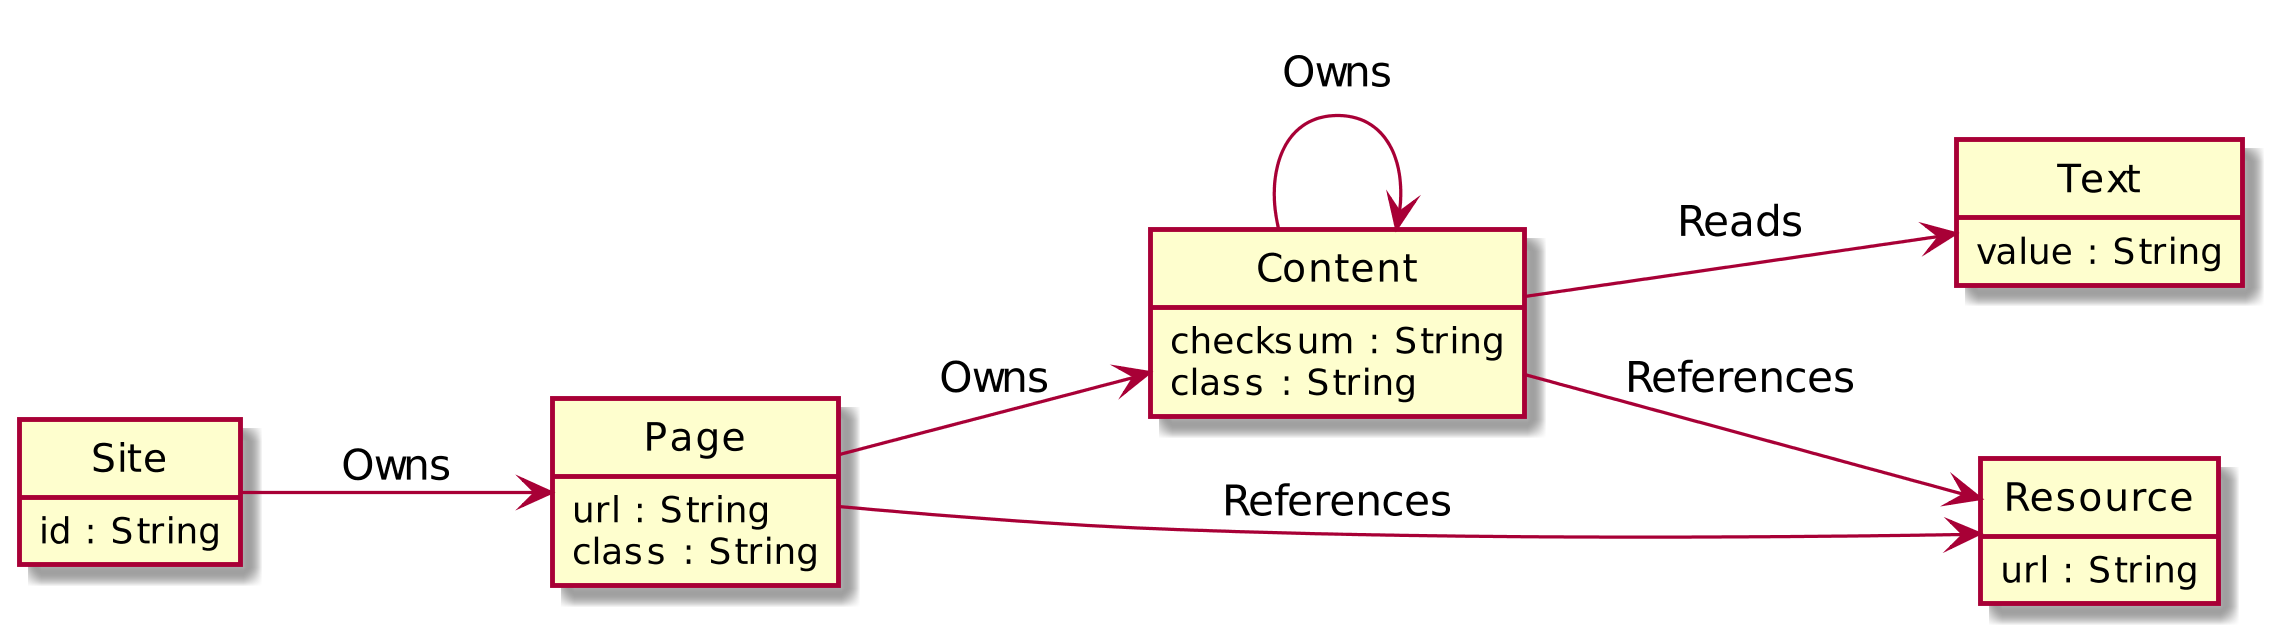
\includegraphics[scale=\imageScalingFactor]{../resources/db-data-model/nodes.png}
        \caption{Übersicht der Nodes und ihrer Beziehungen}
        \label{image:dbDataModelOverview}
    \end{figure}

    Entitäten, die als Node umgesetzt werden, sind Seiten, Content Features,
    der Text eines Content Features, referenzierte {\resources} und Sites.
    Diese erhalten die entsprechenden Labels Page, Content, Text, Reference und Site.
    Eine Seite kann als {\resource} existieren, bevor sie selbst klassifiziert wird.
    In diesem Fall erhält der Knoten zum Zeitpunkt der Klassifizierung zusätzlich auch das Label Page.

    Ein Seitenknoten speichert die \gls{url} der Seite, die auch als eindeutiger Identifier innerhalb der Datenbank dient,
    und die Klasse der Seite.

    Der Knoten einer {\resource} enthält lediglich ihre \gls{url}, die wiederum als eindeutiger Schlüssel dient.
    Wie später deutlich wird, kann er für alle Referenzen, die diese {\resource} als Ziel haben, genutzt werden.

    Knoten mit dem Label "`Content"' enthalten eine Prüfsumme über sich selbst, die innerhalb der Datenbank als Schlüssel Verwendung findet.
    Im späteren Verlauf geht Kapitel \ref{section:solutionDetailsClassificationStorageAPIUpdatePage} darauf ein,
    wieso diese Eigenschaft des Weiteren benötigt wird.
    Für skalare Content Features existiert exakt ein Knoten.
    Für CollectionFeatures existiert ein Knoten pro Element der Liste.

    Der Text eines Content Featuers wird in einem separaten Knoten gespeichert,
    der neben dieser Information nichts speichert und deshalb auch eindeutig über den Text identifiziert wird.
    Zwischen diesen beiden Knoten existiert deshalb eine Beziehung, die das Label Reads besitzt.
    Jeder Content Knoten ist maximal mit einem Textknoten verbunden.
    Der Grund für die Auslagerung ist, dass es viele Features geben kann, die den gleichen textuellen Inhalt besitzen.
    Die Intention ist diese Eigenschaft im Graphen explizit zu machen,
    sodass sie leicht für komplexere Analysen genutzt werden kann.
    Ein Anwendungsfall ist z. B. Informationen aus einer Datenbank,
    die auf verschiedene Seiten ausgegeben werden.
    Ein Text Knoten hat in diesem Fall viele eingehende Beziehungen,
    sodass leicht herausgefunden werden kann, auf welchen Seiten er enthalten ist.
    Eine explizite Beziehung ist dabei semantisch ausdrucksstärker und effizienter,
    als ein einfacher String-Vergleich, der über mit allen Knoten gemacht wird.
    Durch die Beziehung hat man die Info direkt.
    String-Vergleich ist auch dann nicht mehr sinnvoll, wenn man alle Knoten haben möchte,
    die sich einen Text teilen.
    Dann müsste man sehr viele Vergleiche durchführen.
    Durch die Beziehung ist es einfach nur alle Text Nodes, die mehrere einkommende Kanten haben.

    Zu guter Letzt speichern Site Knoten die ID der Site, wodurch der Knoten eindeutig identifiziert wird.
    Jede Seite kann mit beliebig vielen Page Knoten verbunden sein.
    Diese Beziehungen haben das Label Owns.

    Sowohl Seiten als auch Content Features können Content Features enthalten.
    Eine Seite ist zu jedem Content Feature mit einer eigenen Beziehung verbunden,
    die ebenfalls das Label Owns besitzt.
    Das gleiche gilt für Contents und ihre eigenen Content Features.
    Eine genauere Darstellung dieser Beziehung bietet Abbildung \ref{image:dbDataModelContentRelationship}.

    \begin{figure}
        \centering
        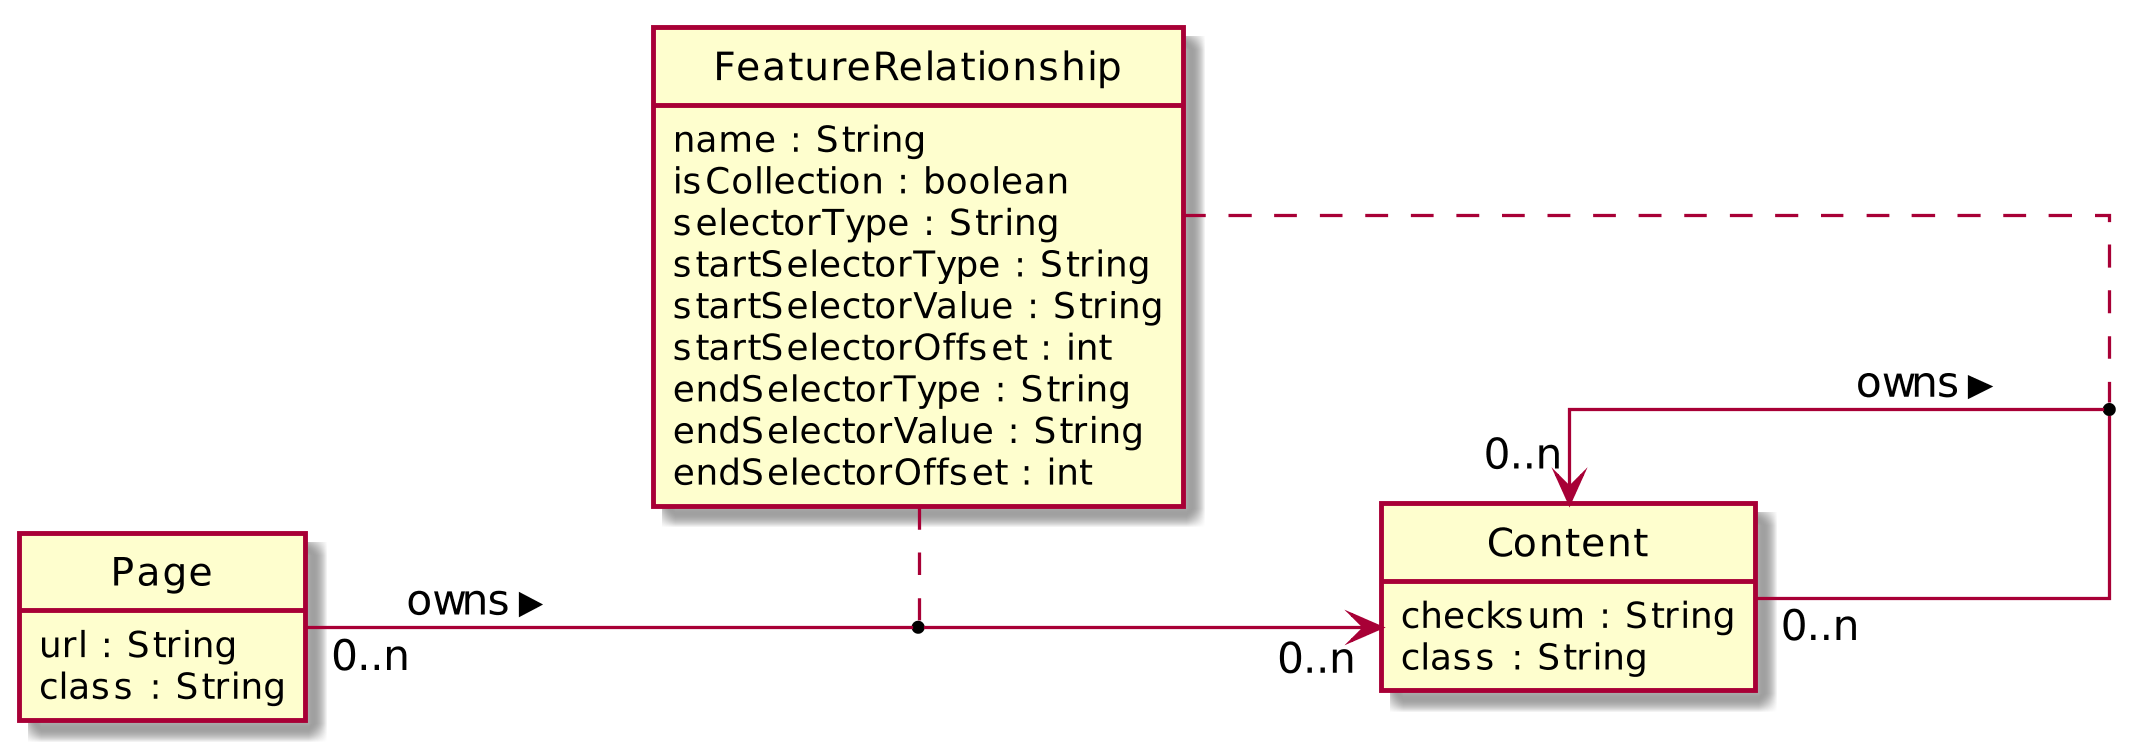
\includegraphics[scale=\imageScalingFactor]{../resources/db-data-model/content-relationship.png}
        \caption{Content Features}
        \label{image:dbDataModelContentRelationship}
    \end{figure}

    Eine Beziehung zwischen Page und Content bzw. Content und Content
    wird hier als FeatureRelationship bezeichnet.
    Eine solche Beziehung besitzt eine Reihe von Eigenschaften.
    Sie speichert den Namen des Features (name),
    ob es sich um ein Element eines CollectionFeatures handelt (isCollection)
    und den eindeutigen Selektor des Nodes, der zum Feature gehört
    (start-, endSelectorType; start-, endSelectorValue; start- endSelectorOffset, ).
    Bei Collection Features existieren viele ausgehende Kanten für ein Feature.
    Jede dieser Beziehungen speichert den gleichen Namen und hat isCollection auf true gesetzt.
    Es ist sinnvoll diese Informationen nicht im Content Knoten, sondern in der Beziehung zu speichern,
    um den Knoten besser wiederverwendbar zu machen.
    Details werden in Kapitel \ref{section:solutionDetailsClassificationStorageAPIUpdatePage} erklärt.

    Referenzen werden in der Datenbank durch eine Kombination aus
    {\resource} Knoten und Beziehungen zu diesen Knoten dargestellt.
    Page und Content Knoten können demanch eine ausgehende Beziehung zu einem
    {\resource} Knoten haben, die mit References markiert ist.
    Abbildung \ref{image:dbDataModelResourceRelationship} stellt diese Beziehung in den Fokus.

    \begin{figure}
        \centering
        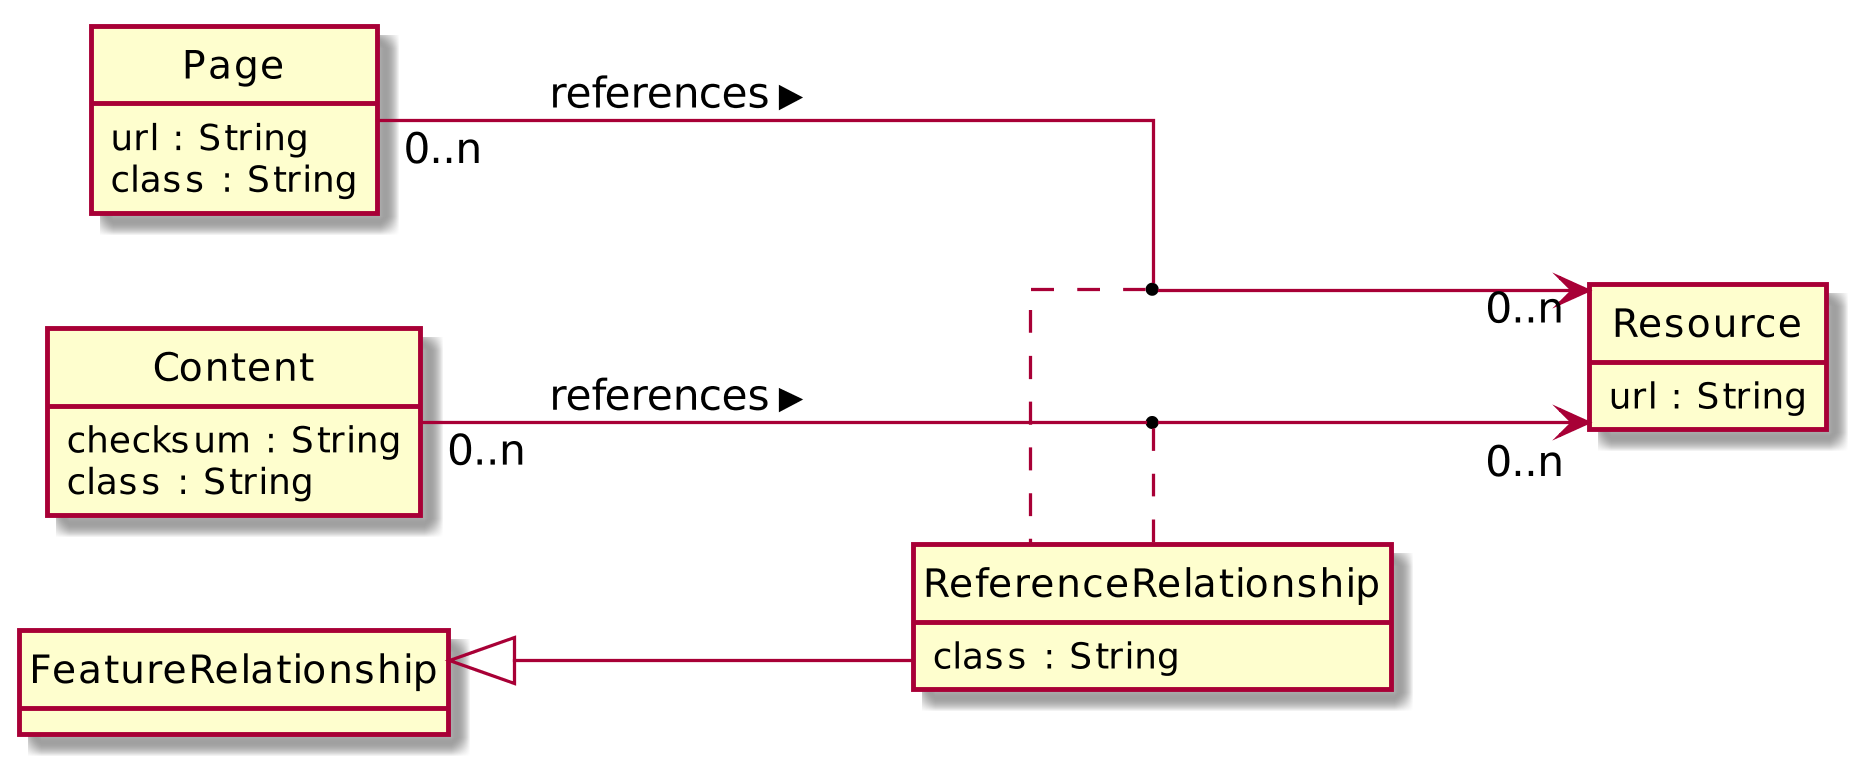
\includegraphics[scale=\imageScalingFactor]{../resources/db-data-model/resource-relationship.png}
        \caption{Reference Features}
        \label{image:dbDataModelResourceRelationship}
    \end{figure}

    Wie zu sehen ist, handelt es sich bei einer ReferenceRelationship ebenfalls
    um eine FeatureRelationship, weshalb sie ebenfalls die oben beschriebenen Informationen speichert.
    Zusätzlich enthält sie aber auch die Klasse der Referenz.
    Diese kann nicht im {\resource} Knoten gespeichert werden,
    da der Knoten für viele Referenzen dienen kann und die Klasse nicht überall identisch sein muss.
    \subsection{Beispiel einer Klassifikation}
    \label{section:solutionDetailPersistenceDataModelExample}
    Um das eben beschriebene Datenmodell greifbarer zu machen,
    präsentiert dieses Kapitel, wie eine konkrete Klassifikation als
    Graph im {\classificationStorage} gespeichert wird.
    Spätere Erklärungen nehmen auf dieses Beispiel ebenfalls Bezug.
    Eine Übersicht der Knoten des Beispielgraphen wurde aus Gründen
    der Übersichtlichkeit auf die Abbildungen \ref{image:dbDataModelExampleOverviewPart1}
    und \ref{image:dbDataModelExampleOverviewPart2} verteilt.
    Sie sind über den \texttt{Content}-Knoten \texttt{c5} verbunden
    und verzichten zunächst auf die ausführliche Darstellung der Eigenschaften der Beziehungen.

    \begin{figure}[htb]
        \centering
        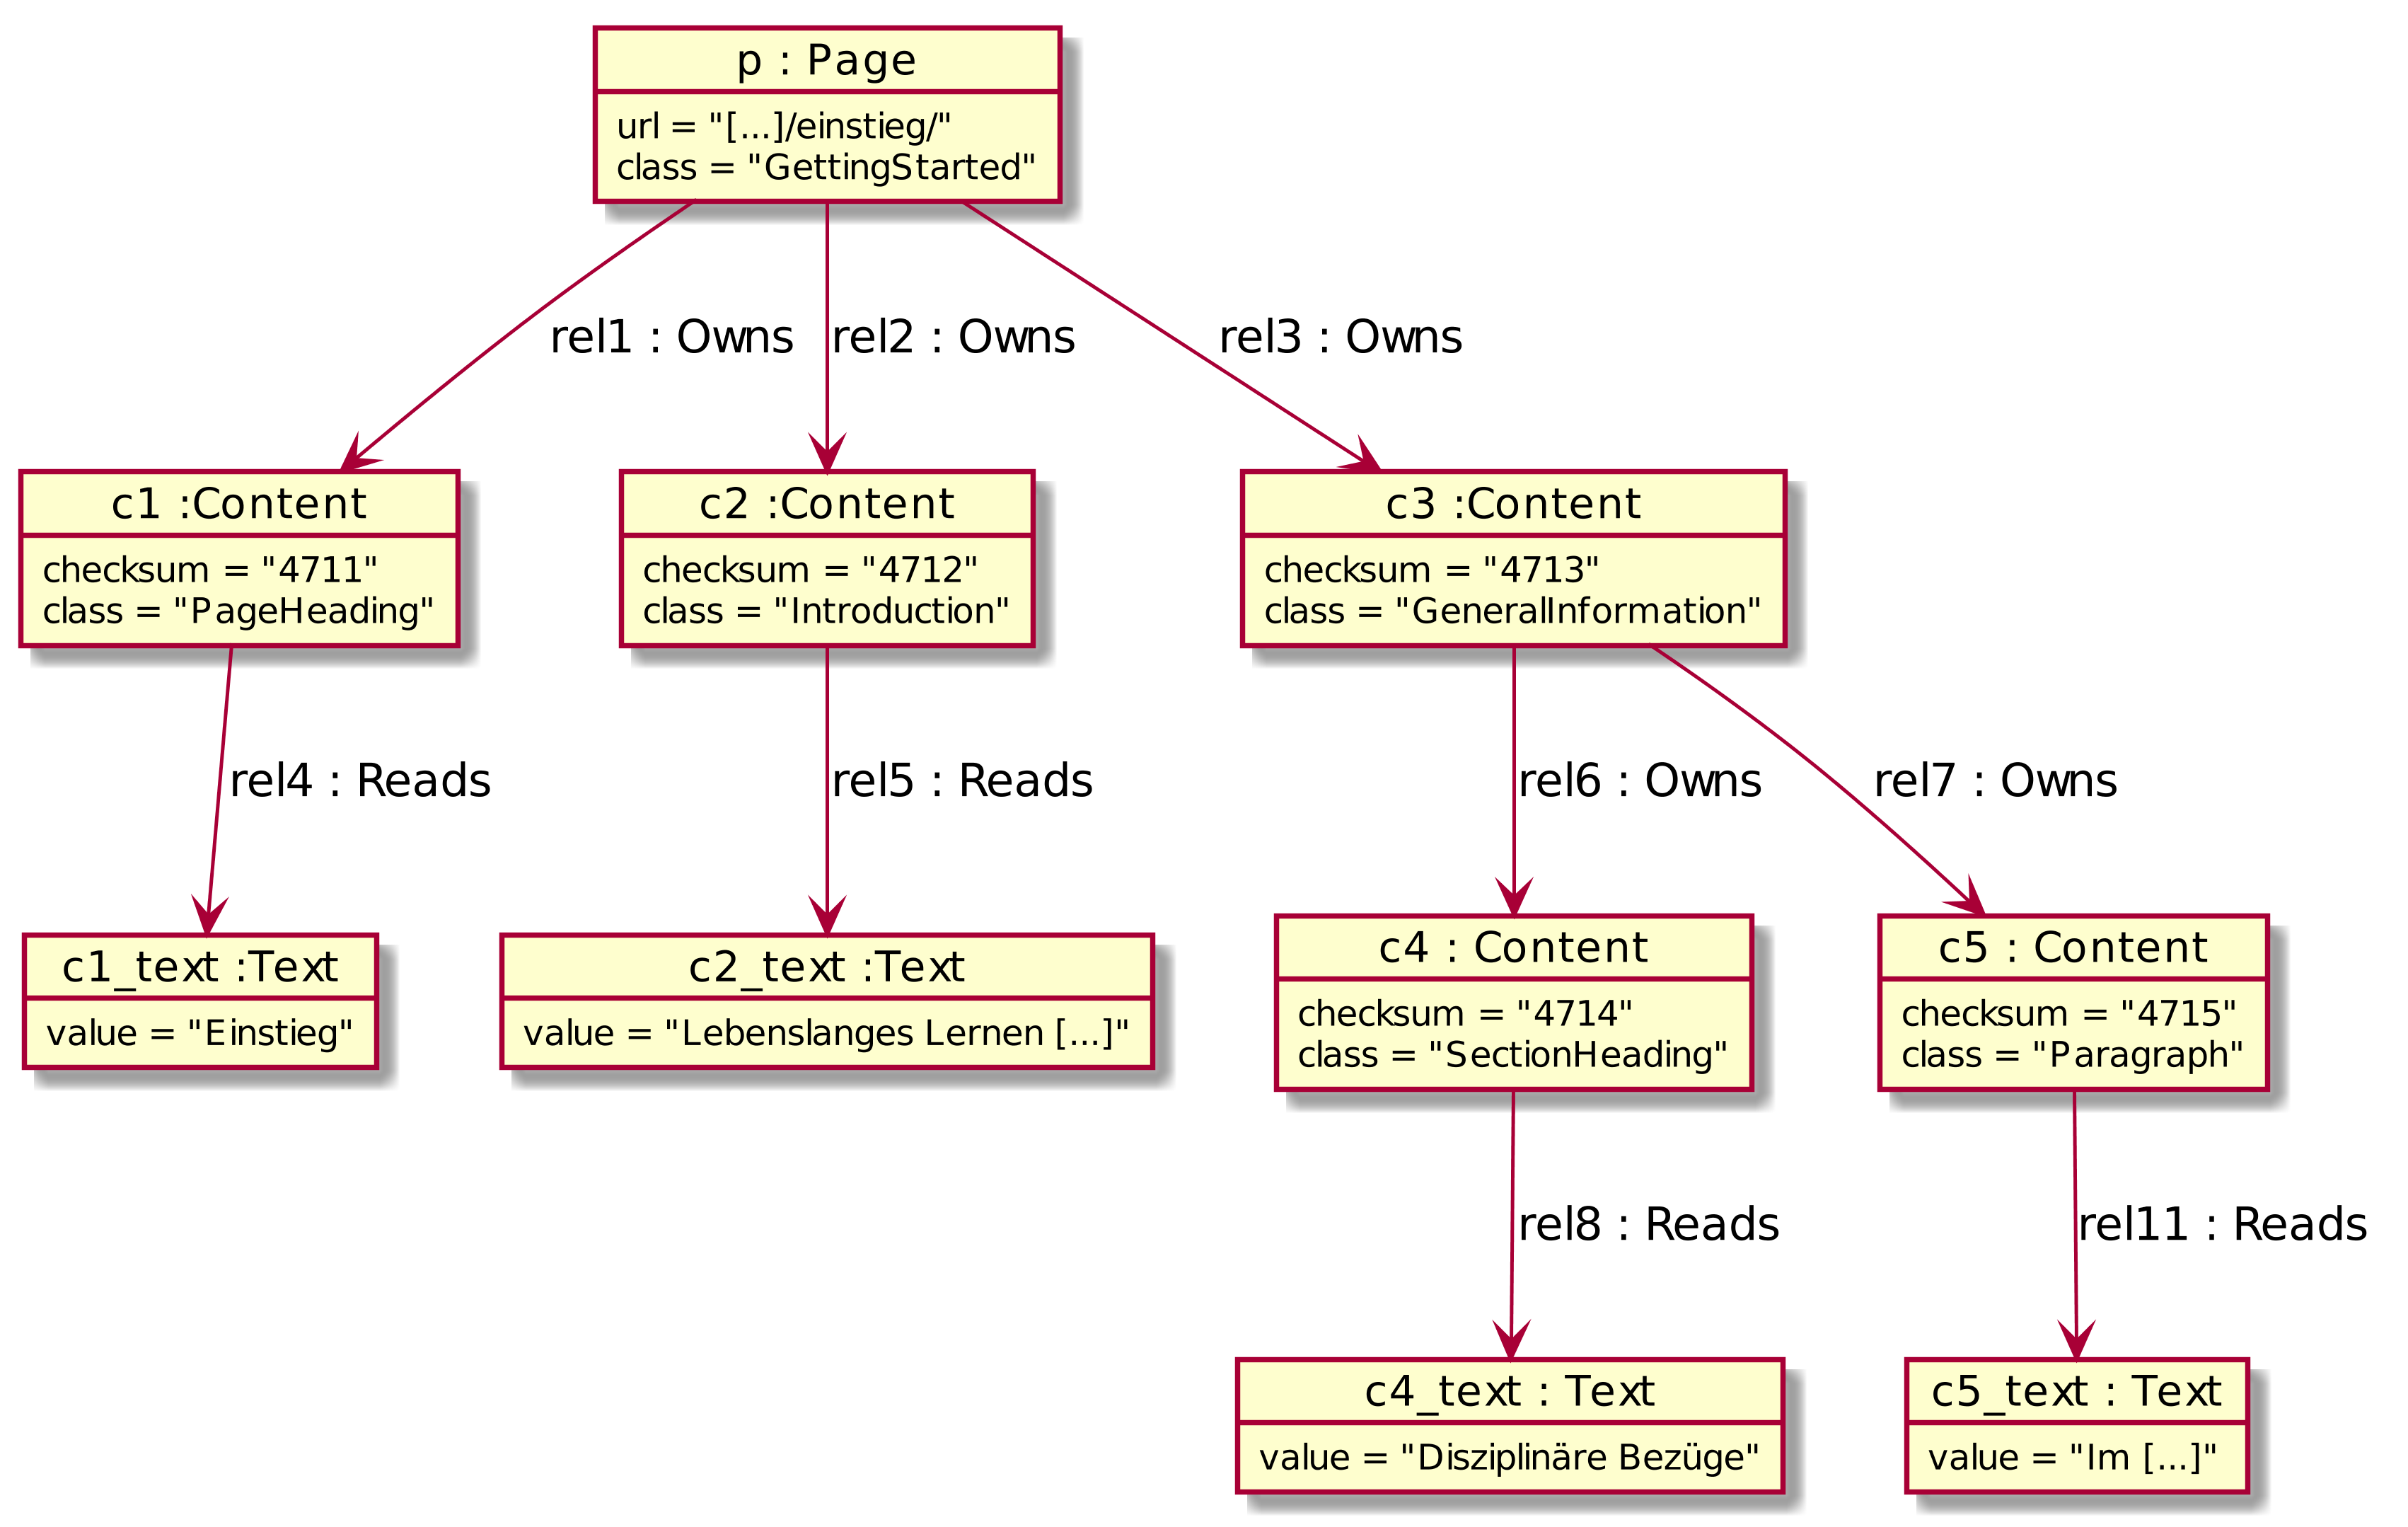
\includegraphics[scale=\imageScalingFactor]{../resources/db-data-model/example/example_part1.png}
        \caption{Ein Beispiel einer Klassifikation im {\classificationStorage} (1)}
        \label{image:dbDataModelExampleOverviewPart1}
    \end{figure}

    Die betroffene Webseite wurde als "`GettingStarted"' klassifiziert und besitzt drei skalare {\contentFeature}s,
    für die \texttt{Content}-Knoten existieren.
    Der \texttt{Page}-Knoten ist mit ihnen über \texttt{Owns}-Beziehungen verbunden.
    Die Inhalte \texttt{c1} und \texttt{c2} beinhalten Text und sind deshalb mit entsprechenden \texttt{Text}-Knoten verbunden.
    Der Knoten \texttt{c3} hat hingegen zwei {\childFeature}s (\texttt{c4} und \texttt{c5}), die seinen Text feingranular speichern
    und deshalb ihrerseits mit \texttt{Text}-Knoten verbunden sind.
    In Abbildung \ref{image:dbDataModelExampleOverviewPart2} ist zu sehen,
    dass \texttt{c5} neben seinem Text auch zwei {\resources} referenziert,
    die durch entsprechende \texttt{Resource}-Knoten dargestellt werden.

    \begin{figure}[htb]
        \centering
        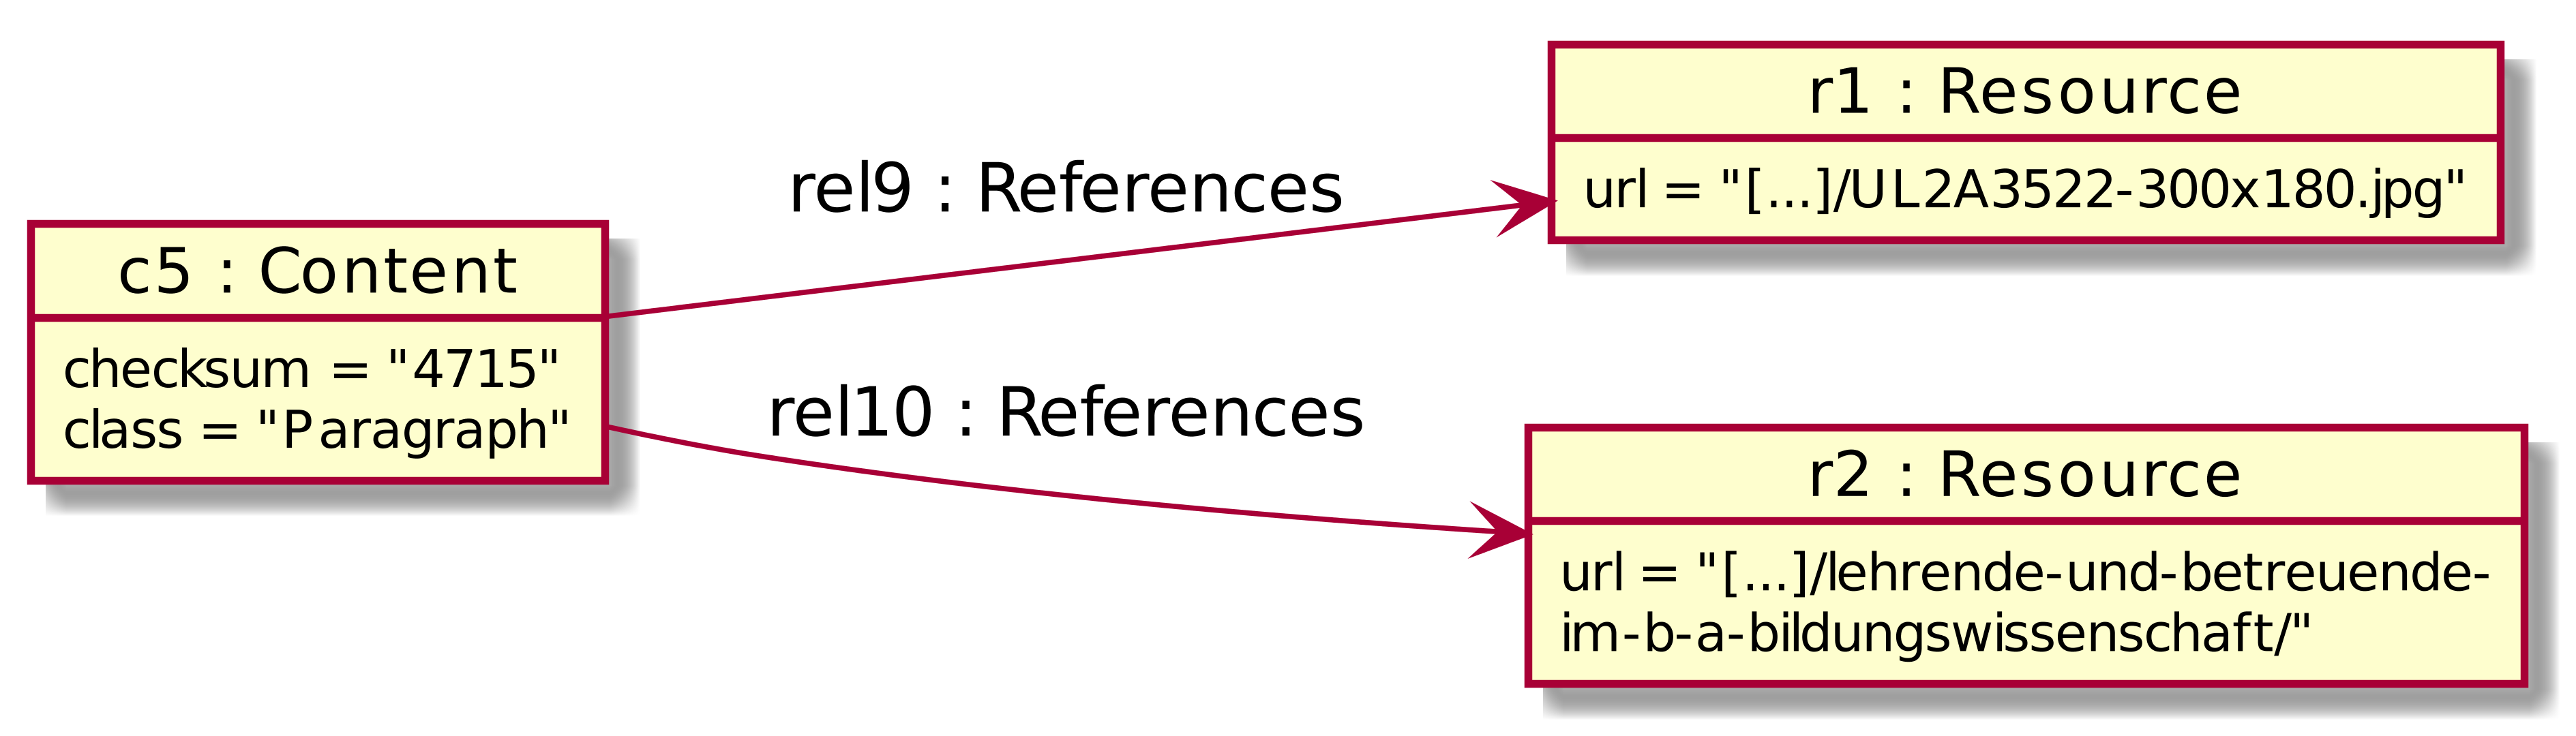
\includegraphics[scale=\imageScalingFactor]{../resources/db-data-model/example/example_part2.png}
        \caption{Ein Beispiel einer Klassifikation im {\classificationStorage} (2)}
        \label{image:dbDataModelExampleOverviewPart2}
    \end{figure}

    Bei diesen Referenzen handelt es sich um ein {\collectionFeature},
    was aus Abbildung \ref{image:dbDataModelExampleRel10} hervorgeht,
    die eine Beziehung zu einem \texttt{Resource}-Knoten detailliert darstellt.

    \begin{figure}[htb]
        \centering
        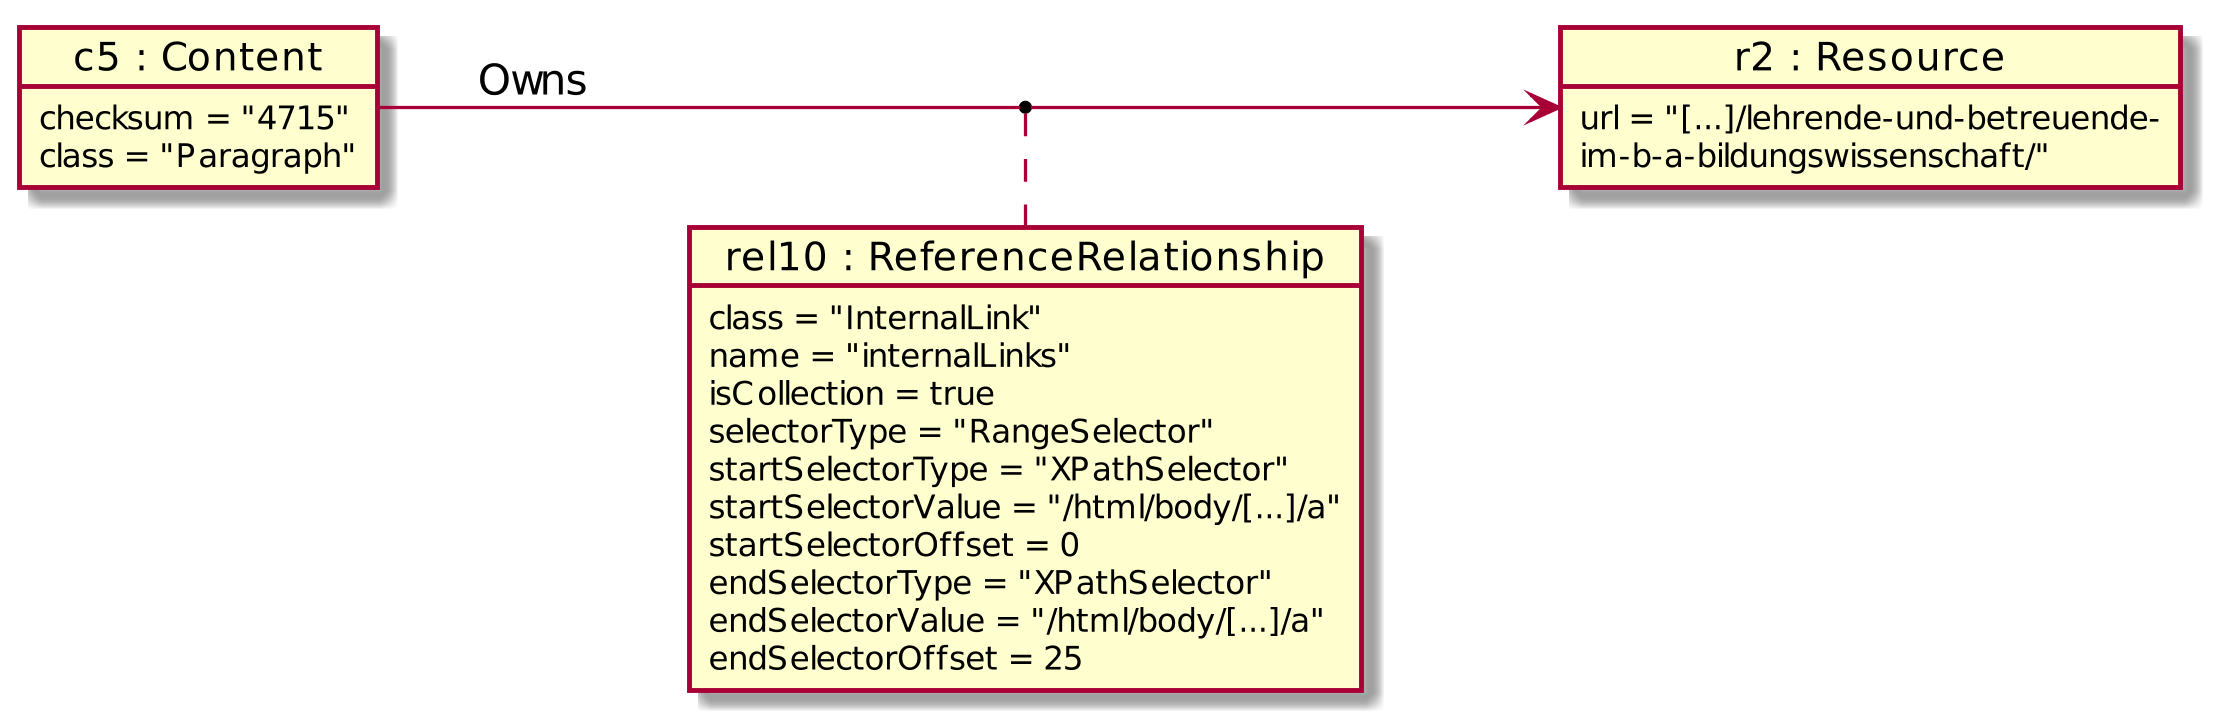
\includegraphics[scale=\imageScalingFactor]{../resources/db-data-model/example/c5-r2.png}
        \caption{Ein Beispiel einer Beziehung zu einem {\resource}-Knoten}
        \label{image:dbDataModelExampleRel10}
    \end{figure}

    Die Eigenschaft \texttt{isCollection} besitzt nämlich den Wert \texttt{true}.
    Des Weiteren wird hier deutlich, wie die Informationen des eindeutigen Selektors gespeichert werden.
    Dem Datenmodell folgend ist eine konkrete Beziehung zu einem \texttt{Content}-Knoten
    sehr ähnlich aufgebaut. Wie in Abbildung \ref{image:dbDataModelExampleRel1} zu sehen,
    verzichtet sie lediglich auf die Speicherung der Klasse.

    \begin{figure}[htb]
        \centering
        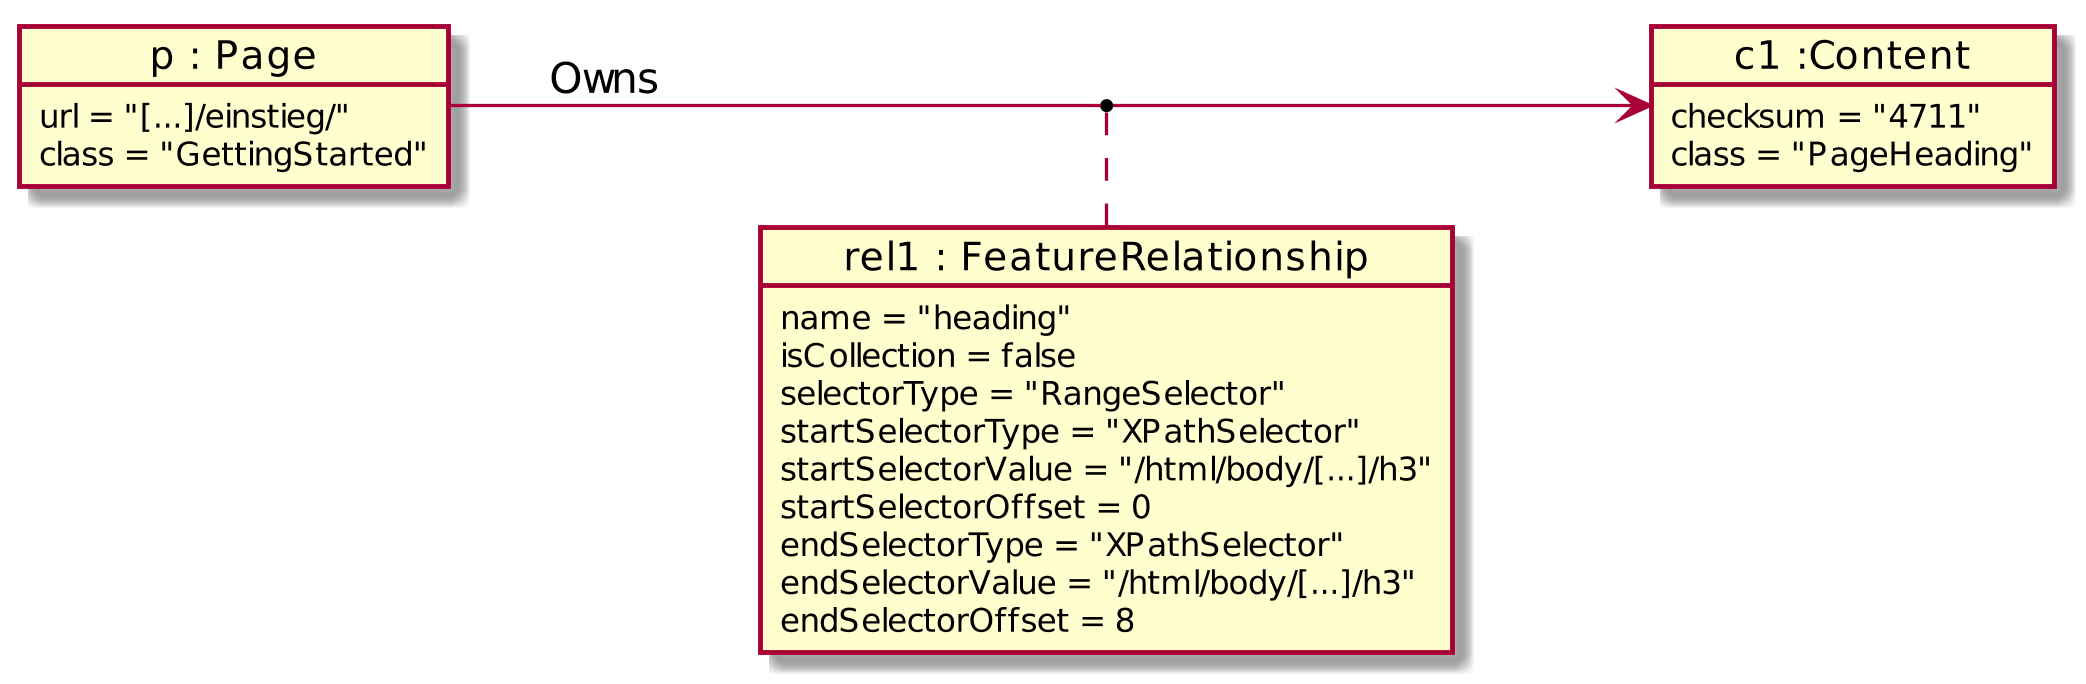
\includegraphics[scale=\imageScalingFactor]{../resources/db-data-model/example/p-c1.png}
        \caption{Ein Beispiel einer Beziehung zu einem Content-Knoten}
        \label{image:dbDataModelExampleRel1}
    \end{figure}

    \subsection{Eignung einer Graphdatenbank}
    Die Nutzung einer Graphdatenbank für das \gls{wccs} hat mehrere Beweggründe.
    Dazu zählen die einfache, natürliche und schemalose Datenmodellierung
    und die Möglichkeit Beziehungen sehr einfach auszuwerten.
    Die Wiederverwendung von Knoten für mehrere Klassifikationen
    bietet außerdem die Möglichkeit, weiterführende Analysen auf den
    klassifizierten Inhalten durchzuführen.
    Dieses Kapitel bewertet die tatsächliche Eignung einer Graphdatenbank,
    des verwendeten Datenmodells sowie des Algorithmus
    zum Schreiben von Klassifikationen, der das Teilen von Knoten ermöglicht.

    \paragraph*{Referenzen zwischen Webseiten}
    Das zweite Fallbeispiel hat gezeigt,
    wie Referenzen zwischen Webseiten auf sehr einfache Art und Weise
    Reihenfolgen und Navigationspfade (der Nachrichtenseiten) explizit machen.
    Eine Auswertung ist trivial, da lediglich ein- und ausgehenden Kanten gefolgt werden muss.
    Andere Datenbankmodelle hätten komplexere Konstrukte
    zur Speicherung und zur Auswertung erfordert.

    \paragraph*{Wiederverwendung von Text- und Resource-Knoten}
    Betrachtet man Tabelle \ref{table:findingsTeachersFiguresNodesByLabel}, wird deutlich,
    dass \texttt{Text}- und \texttt{Resource}-Knoten verhältnismäßig am meisten von der
    Wiederverwendbarkeit Gebrauch machen.
    Das ist nicht verwunderlich, da sie jeweils genau einen Wert speichern,
    der sie identifiziert.
    Gleichzeitig besitzen sie keine ausgehenden Kanten,
    die seitenspezifische Informationen enthalten.
    Wie Tabelle \ref{table:findingsTeachersFiguresSharedNodes} belegt,
    steigt ihre Wiederverwendung bei mehreren Klassifikationen in einer Datenbank,
    was eine logische Konsequenz der größeren Datenmenge ist.
    Für \texttt{Resource}-Knoten ist das aber nicht sofort ersichtlich, da
    die Summe der mehrfach verwendeten \texttt{Resource}-Knoten von Lehrgebieten
    im Falle einzelner Datenbanken höher ist, als im Fall einer gemeinsamen Datenbank (36 vs. 30).
    Gleichzeitig ist die Zahl der geteilten \texttt{SubjectArea}-Knoten aber höher,
    die jeder einen \texttt{Resource}-Knoten eines Lehrgebietes referenzieren.
    Es wird also ein größerer Teil des Graphen wiederverwendet.
    Außerdem enthielten die einzelnen Datenbanken identische \texttt{Resource}-Knoten,
    die in der gemeinsamen natürlich zusammengefasst werden konnten.

    \paragraph*{Entbehrlichkeit von Text-Knoten}
    Innerhalb einer Datenbank macht es aus semantischen Gründen keinen Sinn
    \texttt{Resource}-Knoten zu duplizieren,
    da sie eine Entität der Domäne darstellen.
    {\resources} existieren genau ein mal, was die Datenbank widerspiegeln sollte
    und außerdem die Möglichkeiten eines Graphen besser ausschöpft.
    Nicht so eindeutig ist dies allerdings bei \texttt{Text}-Knoten.
    Aus Tabelle \ref{table:findingsTeachersFiguresSharedNodes} geht hervor,
    dass im ersten Fallbeispiel niemals ein \texttt{Text}-Knoten geteilt wurde.
    Stattdessen konnte immer der zugehörige \texttt{Content}-Knoten geteilt werden.
    Deshalb ist die Zahl beider Knotentypen gesunken und die der geteilten
    \texttt{Content}-Knoten dafür gestiegen.
    Tabelle \ref{table:findingsNewsFiguresSharedNodes}
    zeigt eine andere Situation beim zweiten Fallbeispiel.
    Dort werden zwei \texttt{Text}-Knoten geteilt,
    weil es mehrere Nachrichten mit derselben Überschrift gibt.
    Sie referenzieren aber unterschiedliche Detailseiten,
    weshalb die Nachrichten unterschiedliche \texttt{Content}-Knoten besitzen.
    Der tatsächliche Nutzen der \texttt{Text}-Knoten ist in beiden Beispielen trotzdem sehr gering.
    Der textuelle Wert eines {\contentFeature}s ist deshalb im \texttt{Content}-Knoten selbst besser aufgehoben.
    Für die Schnittstellen des \glspl{wccs} ändert sich durch eine entsprechende Anpassung nichts,
    allerdings vereinfacht sich das Datenmodell der Datenbank sowie
    die generierten Datenbankanweisungen.

    \paragraph*{Hierarchieebene wiederverwendeter Teilgraphen}
    Bezüglich der Wiederverwendung von Teilgraphen ist außerdem ersichtlich,
    dass sie häufig erst auf einer tiefen Ebene des Graphen stattfindet.
    \texttt{Content}-Knoten der Klasse \texttt{SubjectAreaName} werden bspw.
    sehr viel häufiger von mehreren Klassifikationen verwendet als solche der
    Klasse \texttt{Teacher}.
    Betrachtet man die klassifizierten Webseiten,
    ist eine entgegengesetzte Erwartung gerechtfertigt.
    Der Kopfbereich wiederholt sich z. B. auf allen Seiten
    und mehrere Mitarbeiter werden auf unterschiedlichen Webseiten identisch aufgeführt.
    Trotzdem wird bei solchen Mitarbeitern und dem Kopfbereich
    nicht der \texttt{Teacher}- bzw. \texttt{Header}-Knoten geteilt,
    sondern nur ihre Unterknoten.
    Dafür gibt es zwei Gründe.
    Zum einen müssen Features inklusive ihrer {\childFeature}s inhaltlich
    exakt übereinstimmen, damit ihr \texttt{Content}-Knoten mehrfach verwendet werden kann.
    Die kleinste Abweichung macht dies unmöglich,
    da die Inhalte sich letztendlich unterscheiden und nur Teilaspekte übereinstimmen.
    Das muss die Datenbank widerspiegeln.
    Im Falle des Kopfbereiches im ersten Beispiel ist die \gls{url} des Logos
    auf jeder Seite unterschiedlich.
    Das ist im zweiten Beispiel nicht der Fall,
    da alle Seiten zu einem Portal in {\wordpress} gehören
    und deshalb das gleiche Bild referenzieren.
    Deshalb existiert in der Datenbank nur ein \texttt{Header}-Knoten,
    den alle Klassifikationen referenzieren.
    Die zweite Ursache sind unterschiedliche Positionen identischer Inhalte
    auf verschiedenen Webseiten.
    Diese Positionen werden in Form des eindeutigen Selektors in der eingehenden
    Kante eines \texttt{Content}-Knotens gespeichert\footnote{vgl. Kapitel \ref{section:solutionDetailsPersistenceDataModel}}.
    Diese Knoten sind prinzipiell also unabhängig von der konkreten Position
    von mehreren Klassifikationen gleichzeitig nutzbar.
    Dies ändert sich allerdings, sobald ein Inhalt {\childFeature}s besitzt.
    Die ausgehenden Kanten zu diesen Features speichern ihre \textit{absoluten} Selektoren.
    Befindet sich ein Mitarbeiter auf zwei Seiten also nicht an exakt der gleichen Position,
    sind die Selektoren seines Namens, seines Lehrgebietes etc. unterschiedlich.
    Der \texttt{Teacher}-Knoten kann dann nicht von beiden Klassifikationen referenziert
    werden.
    
    \paragraph*{Semantischer Inhalt und physische Struktur einer Webseite}
    Genau betrachtet spiegelt die Datenbank lediglich die Struktur der Webseiten exakt wider.
    Trotzdem lässt sich argumentieren, dass es fachlich konsistenter wäre,
    wenn die \texttt{Teacher}-Knoten im oben beschriebenen Fall geteilt werden würden.
    Ein Beispiel verdeutlicht das:
    Schon jetzt lässt sich die Frage beantworten,
    welche Mitarbeiter in einem gewissen Lehrgebiet arbeiten.
    Dazu muss lediglich den eingehenden Kanten eines
    \texttt{SubjectAreaName}-Knotens über alle \texttt{SubjectArea}-Knoten
    bis zu \texttt{Teacher}-Knoten gefolgt werden.
    Aus fachlicher Sicht ist es aber inkonsistent,
    dass man diese Suche nicht beim \texttt{SubjectArea}-Knoten
    starten kann, weil mehrere dieser Knoten denselben
    \texttt{SubjectAreaName}-Knoten verwenden.
    Aus fachlicher Sicht existieren laut Datenbank also mehrere Lehrgebiete,
    die denselben Namen tragen.
    Hier wird ein Konflikt zwischen dem akkuraten Widerspiegeln der Strukturen der Webseiten
    und dem semantischen Inhalt deutlich.

    \paragraph*{Alternativen}
    Ein erster Schritt zur Auflösung dieses Konfliktes ist, anstatt absolute Selektoren
    lediglich zum {\parentFeature} relative Selektoren in den Kanten zu speichern.
    Allerdings hilft dies nicht, wenn die HTML-Struktur sich unterscheidet,
    weil dann auch die relative Position eines Elementes anders ist.
    Außerdem hätte dies zur Folge, dass zur Ermittlung der eindeutigen Position
    eines Features, der gesamte Vaterpfad bis zur Seite abgelaufen werden muss.
    Eine weitere Alternative zum aktuellen Vorgehen,
    die auch diesen Nachteil umgeht,
    ist die Speicherung der absoluten Selektoren in Kanten,
    die vom \texttt{Page}-Knoten direkt zu \texttt{Content}-Knoten führen.
    Die Teilbarkeit von Content Knoten hinge dann nur noch von den Inhalten und ihrer Klasse ab,
    da die Position komplett unabhängig gespeichert wird.

    \paragraph*{Änderung von Klassifikationen}
    Durch den entwickelten Algorithmus zum Schreiben von Klassifikationen
    wurde das Teilen von Knoten ermöglicht.
    Eine nachteilige Folge ist allerdings,
    dass Änderungen immer über diesen Algorithmus eingearbeitet werden müssen,
    weil sonst Inkonsistenzen riskiert werden.
    Falls die Analysemöglichkeiten keine praktische Relevanz haben,
    ist deshalb ein anderer Datenbanktyp, wie zum Beispiel ein einfacher Document Store,
    in Betracht zu ziehen.

    Insgesamt scheint eine Graphdatenbank trotz der genannten Herausforderungen geeignet
    für den Anwendungsfall des \glspl{wccs}.


    \section{Classification Storage API}
    \label{section:solutionDetailsStorageAPI}
    Wie werden die Daten in die DB geschrieben bzw. gelesen.

    \subsection{Funktionen und Schnitstellen}

    \subsection{Klassifikation speichern}
        \label{section:solutionDetailsStorageAPIStoreClassification}
        \lstinputlisting[label=listing:storeClassification,caption=Algorithmus zum Speichern]{../resources/store-classification.code}

    \subsection{Technologien}
    \section{Annotation Service}
    \begin{table}[htb]
        \centering
        \begin{tabular}{|l|l|}
        \hline
        \textbf{Endpunkt}     & /pages/\{pageId\}\\
        \hline
        \textbf{Methode}      & GET\\
        \hline
        \textbf{Beschreibung} & Liefert Annotator Storage API version\\
        \hline
        \textbf{Status}       & 200\\
        \hline
        \textbf{Antwort}      & \{ ``name'': ``Annotator Store API'', ``version'': ``2.0.0'' \}\\
        \hline
        & \\
        \hline
        \textbf{Endpunkt}     & /pages/\{pageId\}/annotations\\
        \hline
        \textbf{Methode}      & GET\\
        \hline
        \textbf{Beschreibung} & Liefert alle Annotationen einer Seite\\
        \hline
        \textbf{Status}       & 200\\
        \hline
        \textbf{Antwort}      & \{ ``name'': ``Annotator Store API'', ``version'': ``2.0.0'' \}\\
        \hline
        \end{tabular}
        \caption{My caption}
        \label{my-label}
    \end{table}
    % Schnittstellenbeschreibung:
    % - Endpunkt
    % - Methoden
    % -- Input-Dokument
    % -- Status Codes der Antwort
    % -- Return Dokument für jede Antwort
    \section{Das {\annotatorPlugin}}
    \label{section:solutionDetailsAnnotatorPlugin}
    Die Bibliothek Annotator\footnote{vgl. \url{http://annotatorjs.org/}}
    ist ein Open-Source-Produkt zur Anzeige von Webannotationen auf Internetseiten.
    Anders als vergleichbare Produkte wird es nicht nur in der Cloud angeboten,
    sondern kann manuell auf einer Seite eingebunden werden.
    Außerdem besitzt es ein Plugin-System, wodurch es leicht erweitert werden kann.
    Diese Möglichkeit wurde genutzt,
    um das \gls{wccs} in Annotator zu integrieren.

    \subsection{Funktionen und Schnittstellen}
    \label{section:solutionDetailsAnnotationServiceFunctions}
    Der {\annotationService} implementiert vor allem die
    Annotator Storage API \cite[Kapitel "`Storage"']{annotator:documentation},
    um die Nutzung dieser Bibliothek zu ermöglichen.
    Gleichzeitig ist seine Schnittstelle allgemein gehalten,
    sodass sie auch von anderen Systemen sinnvoll genutzt werden kann.
    Die Beschreibung der einzelnen Funktionen erfolgt in diesem Kapitel.

    \paragraph{Format einer Annotation}
    Annotationen tauscht der Service über JSON-Dokumente aus,
    die dem Format von Annotator \cite[Kapitel "`Annotation format"' ]{annotator:documentation} folgen.
    Der Service ergänzt aber einige Angaben.
    Das Schema einer Annotation zeigt Listing \ref{listing:annotationServiceAnnotationFormat}.

    \lstinputlisting[
        label=listing:annotationServiceAnnotationFormat,
        caption=Das Format einer Annotation,
        style=json
    ]{../resources/annotation-service/annotation.json}

    Jede Annotation spiegelt genau ein Feature der Klassifikation wider.
    Die ID einer Annotation wird vom {\annotationService} automatisch
    generiert.
    Das Feld \texttt{text} bestimmt den Inhalt der Annotation,
    der hier immer der Namen des Features und dessen Klasse ist.
    Die Angaben im Feld \texttt{ranges} spiegeln den eindeutigen Selektor des Features wider.
    Durch das Feld \texttt{user} identifiziert Annotator den Ersteller der Annotation,
    der in diesem Fall immer der imaginäre technische Benutzer \texttt{wccs} ist.
    Im Feld \texttt{permissions} werden die Rechte \texttt{admin} und \texttt{delete} auf diesen Nutzer beschränkt.
    Jeder Anwender kann dadurch Annotation lesen und bearbeiten.
    Änderungen an den Rechten sowie das Löschen einer Annotation bleibt aber dem Nutzer \texttt{wccs} vorbehalten.
    Die Eigenschaft \texttt{wccs} ist nicht durch Annotator vorgegeben,
    sondern stellt eine Ergänzung des \glspl{wccs} dar.
    Es speichert die Klasse und Art (Inhalt oder Referenz) eines Features.

    \paragraph{Bereitstellung von Informationen über die Schnittstelle}
    Um der Annotator Storage API \cite[Kapitel "`Storage"' ]{annotator:documentation} zu genügen,
    muss ein Endpunkt existieren,
    der Informationen über die Version der implementierten Schnittstelle
    enthält.
    Die entsprechende Schnittstelle ist in Tabelle
    \ref{table:annotationServiceMetaInterface} dokumentiert.

    \begin{table}[htb]
        \centering
        \begin{tabular}{|l|l|}
            \hline
            \textbf{\gls{url}} & \texttt{http://<HOST>:16612/pages/<PAGE\_ID>}\\
            \hline
            \textbf{Methode} & \texttt{GET}\\
            \hline
            \textbf{Statuscode} & \texttt{200 (OK)}\\
            \hline
            \textbf{Ausgabedokument} & \lstinputlisting[title=AnnotationServiceMetaInfo]{../resources/annotation-service/meta.json}\\
            \hline
        \end{tabular}
        \caption{Die Schnittstelle zum Abfragen von Informationen über den {\annotationService}}
        \label{table:annotationServiceMetaInterface}
    \end{table}

    Annotator erwartet von der konfigurierten Datenhaltung,
    dass sie die Annotationen genau einer Seite enthält.
    Die Anfrage-\gls{url} enthält deshalb die \gls{url} der klassifizierten Webseite,
    deren Annotationen angefordert werden.

    \paragraph{Annotationen einer Seite abrufen}
    Zentrale Aufgabe des {\annotationService}s ist die Bereitstellung der Annotationen einer Seite.
    Hierfür bietet der Service die in Tabelle \ref{table:getAllAnnotationsInterface}
    dargestellte Schnittstelle.

    \begin{table}[htb]
        \centering
        \begin{tabular}{|l|l|}
            \hline
            \textbf{\gls{url}} & \texttt{http://<HOST>:16612/pages/<PAGE\_ID>/annotations}\\
            \hline
            \textbf{Methode} & \texttt{GET}\\
            \hline
            \textbf{Statuscode} & \texttt{200 (OK)}\\
            \hline
            \textbf{Ausgabedokument} & \texttt{Array von Annotationen}\\
            \hline
        \end{tabular}
        \caption{Die Schnittstelle zum Abfragen aller Annotationen einer Klassifikation}
        \label{table:getAllAnnotationsInterface}
    \end{table}

    Die Anfrage-\gls{url} identifiziert die klassifizierte Seite,
    an deren Annotationen Interesse besteht,
    über ihre \gls{url}.
    Die Antwort des Services ist ein Array von Annotationen, wie sie im ersten Abschnitt vorgestellt wurden.

    \paragraph{Einzelne Annotation abfragen}
    Über die Schnittstelle in Tabelle \ref{table:getAnnotationInterface} kann eine einzelne
    Annotation anhand ihrer ID angefragt werden.

    \begin{table}[htb]
        \centering
        \begin{tabular}{|l|l|}
            \hline
            \textbf{\gls{url}} & \texttt{http://<HOST>:16612/pages/<PAGE\_ID>/annotations/<ANNOTATION\_ID>}\\
            \hline
            \textbf{Methode} & \texttt{GET}\\
            \hline
            \textbf{Statuscode} & \texttt{200 (OK)}\\
            \hline
            \textbf{Ausgabedokument} & \texttt{Annotation}\\
            \hline
        \end{tabular}
        \caption{Die Schnittstelle zum Abfragen einer einzelnen Annotation}
        \label{table:getAnnotationInterface}
    \end{table}

    \paragraph{Einzelne Annotation aktualisieren}
    Änderungen an einer Annotation können dem {\annotationService} über die Schnittstelle
    in Tabelle \ref{table:putAnnotationInterface} mitgeteilt werden.
    Als Resultat wird die Klasse des verknüpften Features
    überschrieben.

    \begin{table}[htb]
        \centering
        \begin{tabular}{|l|l|}
            \hline
            \textbf{\gls{url}} & \texttt{http://<HOST>:16612/pages/<PAGE\_ID>/annotations/<ANNOTATION\_ID>}\\
            \hline
            \textbf{Methode} & \texttt{PUT}\\
            \hline
            \textbf{Eingabedokument} & \texttt{Annotation}\\
            \hline
            \textbf{Statuscode} & \texttt{303 (See Other)}\\
            \hline
        \end{tabular}
        \caption{Die Schnittstelle zum Schreiben einer Annotation}
        \label{table:putAnnotationInterface}
    \end{table}

    Die Anfrage muss eine Annotation im oben beschriebenen Format enthalten.
    Die Antwort des Services enthält im Header \texttt{Location} die \gls{url} der geschriebenen Annotation.

    % TODO: Schnittstelle so, dass später auch anderes Format für Annotationen möglich
    \subsection{Einbindung des Plugins}
    Das Plugin kann prinzipiell in jede beliebige Webseite eingebunden werden,
    die Annotator verwendet.
    Dazu sind die folgenden Schritte notwendig.

    \paragraph{Einbinden von Annotator}
    Zunächst muss gewährleistet sein, dass die
    Annotator Bibliothek\footnote{\url{http://assets.annotateit.org/annotator/v1.2.10/annotator-full.min.js}}
    und die Annotator Stylesheets\footnote{\url{http://assets.annotateit.org/annotator/v1.1.0/annotator.min.css}}
    korrekt in die Seite eingebunden sind.

    \paragraph{Einbinden des \gls{wccs}-Annotator-Plugins}
    Des Weiteren muss das Annotator Plugin des \gls{wccs} im head der Seite über ein
    script Tag engebunden werden.

    \paragraph{Einbinden weiterer Style-Definitionen}
    Anschließend sollten die Styledefinition aus Listing \ref{listing:annotatorCustomStyles}
    dem head der Webseite hinzugefügt werden,
    da Annotator das HTML der Seite bearbeitet und andernfalls Designprobleme auftreten können.

    \lstinputlisting[
        label=listing:annotatorCustomStyles,
        caption=Eigene Styles für Annotator,
        style=pseudo
    ]{../resources/annotator-plugin/custom-styles.html}

    \paragraph{Annotator Initialisierung}
    Anschließend muss der Initialisierungsaufruf von Annotator ergänzt werden,
    sodass Annotator das neue Plugin verwendet.
    Listing \ref{listing:annotatorInitialization} zeigt eine Beispielhafte
    Initialisierung von Annotator, die das \gls{wccs}-Plugin integriert.

    \lstinputlisting[
        label=listing:annotatorInitialization,
        caption=Angepasste Annotator-Initialisierung,
        style=pseudo
    ]{../resources/annotator-plugin/annotator-initialize.js}

    Nachdem Annotator auf dem body der Webseite initialisiert wurde,
    werden die verschiedenen Plugins registriert.
    Begonnen wird mit dem
    Storage Plugin\footnote{vgl. \url{http://docs.annotatorjs.org/en/v1.2.x/plugins/store.html}},
    welches für den Annotation Service konfiguriert wird.
    Entsprechend der vorgestellten Schnittstelle dieser
    Komponente\footnote{vgl. Kapitel \ref{section:solutionDetailsAnnotationServiceFunctions}}
    legt die Konfiguration des Plugins den Präfix von Anfrage-\glspl{url} fest.
    Diese beinhaltet die kodierte \gls{url} der aktuellen Seite,
    welche als Schlüssel der Seite fungiert.
    Anschließend wird das \gls{wccs}-Annotator-Plugin über den Schlüssel "`wccs"' inkludiert.
    Zuletzt konfiguriert das Skript das
    Permissions Plugin\footnote{vgl. \url{http://docs.annotatorjs.org/en/v1.2.x/plugins/permissions.html}}.

    \section{Die Webanwendung}
    Die Webanwendung zur ausführlicheren Einsicht
    und Prüfungen von Klassifikationen steht im Mittelpunkt dieses Kapitels.

    \subsection{Funktionen und Schnittstellen}
    \label{section:solutionDetailsAnnotationServiceFunctions}
    Der {\annotationService} implementiert vor allem die
    Annotator Storage API \cite[Kapitel "`Storage"']{annotator:documentation},
    um die Nutzung dieser Bibliothek zu ermöglichen.
    Gleichzeitig ist seine Schnittstelle allgemein gehalten,
    sodass sie auch von anderen Systemen sinnvoll genutzt werden kann.
    Die Beschreibung der einzelnen Funktionen erfolgt in diesem Kapitel.

    \paragraph{Format einer Annotation}
    Annotationen tauscht der Service über JSON-Dokumente aus,
    die dem Format von Annotator \cite[Kapitel "`Annotation format"' ]{annotator:documentation} folgen.
    Der Service ergänzt aber einige Angaben.
    Das Schema einer Annotation zeigt Listing \ref{listing:annotationServiceAnnotationFormat}.

    \lstinputlisting[
        label=listing:annotationServiceAnnotationFormat,
        caption=Das Format einer Annotation,
        style=json
    ]{../resources/annotation-service/annotation.json}

    Jede Annotation spiegelt genau ein Feature der Klassifikation wider.
    Die ID einer Annotation wird vom {\annotationService} automatisch
    generiert.
    Das Feld \texttt{text} bestimmt den Inhalt der Annotation,
    der hier immer der Namen des Features und dessen Klasse ist.
    Die Angaben im Feld \texttt{ranges} spiegeln den eindeutigen Selektor des Features wider.
    Durch das Feld \texttt{user} identifiziert Annotator den Ersteller der Annotation,
    der in diesem Fall immer der imaginäre technische Benutzer \texttt{wccs} ist.
    Im Feld \texttt{permissions} werden die Rechte \texttt{admin} und \texttt{delete} auf diesen Nutzer beschränkt.
    Jeder Anwender kann dadurch Annotation lesen und bearbeiten.
    Änderungen an den Rechten sowie das Löschen einer Annotation bleibt aber dem Nutzer \texttt{wccs} vorbehalten.
    Die Eigenschaft \texttt{wccs} ist nicht durch Annotator vorgegeben,
    sondern stellt eine Ergänzung des \glspl{wccs} dar.
    Es speichert die Klasse und Art (Inhalt oder Referenz) eines Features.

    \paragraph{Bereitstellung von Informationen über die Schnittstelle}
    Um der Annotator Storage API \cite[Kapitel "`Storage"' ]{annotator:documentation} zu genügen,
    muss ein Endpunkt existieren,
    der Informationen über die Version der implementierten Schnittstelle
    enthält.
    Die entsprechende Schnittstelle ist in Tabelle
    \ref{table:annotationServiceMetaInterface} dokumentiert.

    \begin{table}[htb]
        \centering
        \begin{tabular}{|l|l|}
            \hline
            \textbf{\gls{url}} & \texttt{http://<HOST>:16612/pages/<PAGE\_ID>}\\
            \hline
            \textbf{Methode} & \texttt{GET}\\
            \hline
            \textbf{Statuscode} & \texttt{200 (OK)}\\
            \hline
            \textbf{Ausgabedokument} & \lstinputlisting[title=AnnotationServiceMetaInfo]{../resources/annotation-service/meta.json}\\
            \hline
        \end{tabular}
        \caption{Die Schnittstelle zum Abfragen von Informationen über den {\annotationService}}
        \label{table:annotationServiceMetaInterface}
    \end{table}

    Annotator erwartet von der konfigurierten Datenhaltung,
    dass sie die Annotationen genau einer Seite enthält.
    Die Anfrage-\gls{url} enthält deshalb die \gls{url} der klassifizierten Webseite,
    deren Annotationen angefordert werden.

    \paragraph{Annotationen einer Seite abrufen}
    Zentrale Aufgabe des {\annotationService}s ist die Bereitstellung der Annotationen einer Seite.
    Hierfür bietet der Service die in Tabelle \ref{table:getAllAnnotationsInterface}
    dargestellte Schnittstelle.

    \begin{table}[htb]
        \centering
        \begin{tabular}{|l|l|}
            \hline
            \textbf{\gls{url}} & \texttt{http://<HOST>:16612/pages/<PAGE\_ID>/annotations}\\
            \hline
            \textbf{Methode} & \texttt{GET}\\
            \hline
            \textbf{Statuscode} & \texttt{200 (OK)}\\
            \hline
            \textbf{Ausgabedokument} & \texttt{Array von Annotationen}\\
            \hline
        \end{tabular}
        \caption{Die Schnittstelle zum Abfragen aller Annotationen einer Klassifikation}
        \label{table:getAllAnnotationsInterface}
    \end{table}

    Die Anfrage-\gls{url} identifiziert die klassifizierte Seite,
    an deren Annotationen Interesse besteht,
    über ihre \gls{url}.
    Die Antwort des Services ist ein Array von Annotationen, wie sie im ersten Abschnitt vorgestellt wurden.

    \paragraph{Einzelne Annotation abfragen}
    Über die Schnittstelle in Tabelle \ref{table:getAnnotationInterface} kann eine einzelne
    Annotation anhand ihrer ID angefragt werden.

    \begin{table}[htb]
        \centering
        \begin{tabular}{|l|l|}
            \hline
            \textbf{\gls{url}} & \texttt{http://<HOST>:16612/pages/<PAGE\_ID>/annotations/<ANNOTATION\_ID>}\\
            \hline
            \textbf{Methode} & \texttt{GET}\\
            \hline
            \textbf{Statuscode} & \texttt{200 (OK)}\\
            \hline
            \textbf{Ausgabedokument} & \texttt{Annotation}\\
            \hline
        \end{tabular}
        \caption{Die Schnittstelle zum Abfragen einer einzelnen Annotation}
        \label{table:getAnnotationInterface}
    \end{table}

    \paragraph{Einzelne Annotation aktualisieren}
    Änderungen an einer Annotation können dem {\annotationService} über die Schnittstelle
    in Tabelle \ref{table:putAnnotationInterface} mitgeteilt werden.
    Als Resultat wird die Klasse des verknüpften Features
    überschrieben.

    \begin{table}[htb]
        \centering
        \begin{tabular}{|l|l|}
            \hline
            \textbf{\gls{url}} & \texttt{http://<HOST>:16612/pages/<PAGE\_ID>/annotations/<ANNOTATION\_ID>}\\
            \hline
            \textbf{Methode} & \texttt{PUT}\\
            \hline
            \textbf{Eingabedokument} & \texttt{Annotation}\\
            \hline
            \textbf{Statuscode} & \texttt{303 (See Other)}\\
            \hline
        \end{tabular}
        \caption{Die Schnittstelle zum Schreiben einer Annotation}
        \label{table:putAnnotationInterface}
    \end{table}

    Die Anfrage muss eine Annotation im oben beschriebenen Format enthalten.
    Die Antwort des Services enthält im Header \texttt{Location} die \gls{url} der geschriebenen Annotation.

    % TODO: Schnittstelle so, dass später auch anderes Format für Annotationen möglich
    \subsection{Technologien}
    Der Service beinhaltet einen nginx Webserver\footnote{vgl. \url{https://nginx.org}},
    der die Webanwendung über Port 80 bereitstellt.
    Diese verwendet das Webapplikationsframework Angular\footnote{https://angular.io}
    und ist in TypeScript geschrieben.
    Des Weiteren verwendet es die Bibliotheken
    Bootstrap\footnote{vgl. \url{https://getbootstrap.com/}}
    und ng-bootstrap\footnote{vgl. \url{https://ng-bootstrap.github.io}}.

    \section{Der {\wordpressCrawler}}
    \label{section:solutionDetailsCrawler}
    Das \gls{wccs} beinhaltet eine Beispielimplementierung für ein Werkzeug,
    welches für eine Menge an Webseiten Klassifizierungsaufträge absetzt.
    Dabei handelt es sich um den {\wordpressCrawler},
    der über {\wordpress}' RESTful Webservice \cite{wordpress:RestAPI}
    die \glspl{url} aller Beiträge und Seiten ermittelt
    und an den {\classificationService}\footnote{vgl. Kapitel \ref{section:solutionDetailsClassificationService}}
    zur Klassifizierung weitergibt.
    Im Folgenden wird die Konfiguration und Nutzung dieses Kommandozeilenwerkzeugs beschrieben.

    \subsection{Konfiguration und Aufruf}
    Der {\wordpressCrawler} benötigt zur Ausführung einige Informationen,
    die ihm beim Start in einer Konfigurationsdatei mitgeteilt werden.
    Diese Parameter lassen sich in drei Kategorien einteilen:
    Classification Service, Sites und Crawling.

    \paragraph{Parameter der Kategorie Classification Service}
    Da der {\wordpressCrawler} kein Service des \glspl{wccs} ist,
    muss ihm die \gls{url} eines laufenden {\classificationService}s mitgeteilt werden,
    an den er die Klassifizierungsaufträge richten soll.
    Die verfügbaren Parameter hierfür sind in Tabelle \ref{table:crawlerClassificationServiceParameter} aufgeführt.
    Jeder dieser Parameter ist optional und besitzt deshalb einen Standardwert.

    \begin{table}[]
        \centering
        \begin{tabular}{|l|l|}
            \hline
            \textbf{Parameter} & \textbf{Standardwert}\\
            \hline
            \texttt{scheme} & \texttt{http} \\
            \hline
            \texttt{host} & \texttt{localhost} \\
            \hline
            \texttt{port} & \texttt{44284} \\
            \hline
            \texttt{path} & \texttt{/classifications} \\
            \hline
            \end{tabular}
        \caption{Die Konfigurationsparameter des {\wordpressCrawler}s für den {\classificationService}}
        \label{table:crawlerClassificationServiceParameter}
    \end{table}

    Der {\wordpressCrawler} baut die \gls{url} des {\classificationService}s nach
    folgendem Schema auf: \texttt{<scheme>://<host>:<port>:<path>}.

    \paragraph{Parameter der Kategorie Sites}
    Darüber hinaus muss das Werkzeug wissen,
    welche {\wordpress} Sites es durchsuchen soll.
    Diese Information wird ebenfalls in der Konfiguration gespeichert.
    Eine {\wordpress} Site wird darin durch
    ihre \gls{url}, einen Namen und eine frei wählbare eindeutige ID definiert.

    \paragraph{Parameter der Kategorie Crawling}
    Diese Kategorie der Konfiguration kennt zwei weitere Parameter:
    \texttt{resultPageSize} und \texttt{maxConcurrentRequests}.
    Der erste Parameter legt die Anzahl der Beiträge und Seiten fest,
    die der {\wordpressCrawler} in einer Anfrage von {\wordpress} anfordert.
    Der Standardwert dieses Parameters ist 8.
    Der zweite Parameter bestimmt die Anzahl der gleichzeitigen Anfragen,
    die vom Crawler an {\wordpress} gerichtet werden.
    Hier liegt der Standardwert bei 5.
    Beide Parameter dienen der Erzeugung eines guten Flusses und stellen sicher,
    dass {\wordpress} durch die Anfragen des Crawlers
    nicht überlastet wird und keine anderen Anfragen mehr bearbeiten kann.

    \paragraph{Beispielkonfiguration}
    Eine konkrete Konfiguration muss in YAML\footnote{vgl. \url{http://yaml.org}} geschrieben sein.
    Ein Beispiel ist in Listing \ref{listing:crawlerConfiguration} zu sehen.

    \lstinputlisting[
        label=listing:crawlerConfiguration,
        caption=Eine Beispielkonfiguration des {\wordpressCrawler}s,
        style=crawlerConfig
    ]{../resources/crawler/config.yaml}

    \paragraph{Aufruf}
    Der Aufruf des {\wordpressCrawler}s erfolgt über automatisch generierte Startskripte,
    die dem Werkzeug beiliegen.
    Als Argument muss ihnen der Pfad zur Konfigurationsdatei übergeben werden.
    Ein beispielhafter Aufruf ist \texttt{./wccs-wordpress-crawler /home/wccs/crawler.yaml}.

    \subsection{Technologien}
    Der Service beinhaltet einen nginx Webserver\footnote{vgl. \url{https://nginx.org}},
    der die Webanwendung über Port 80 bereitstellt.
    Diese verwendet das Webapplikationsframework Angular\footnote{https://angular.io}
    und ist in TypeScript geschrieben.
    Des Weiteren verwendet es die Bibliotheken
    Bootstrap\footnote{vgl. \url{https://getbootstrap.com/}}
    und ng-bootstrap\footnote{vgl. \url{https://ng-bootstrap.github.io}}.

    \section{Plattform}
    Die verschiedenen Services des \gls{wccs} sind als
    setzen auf der Docker Plattform\footnote{vgl. \url{https://www.docker.com}} auf,
    wodurch sie von einander isoliert betrieben werden sowie einfach einzeln
    gestoppt, gestartet und skaliert werden können.

    Konkret laufen
    der Annotation Service,
    der Classification Service,
    der Classification Storage,
    die Classification Storage API,
    und die Webanwendung in Docker Containern.
    Diese werden über das Tool Docker Compose\footnote{vgl. \url{https://docs.docker.com/compose}}
    gebaut, ausgeführt und über ein virtuelles Netzwerk verbunden.
    Die enthaltene Konfiguration mappt die Ports der Services
    1:1 auf die gleichen Ports des Host-Systems.

